\chapter{Source Code}
%% Create a new environment for breaking code listings across pages.
\newenvironment{longlisting}{\captionsetup{type=listing}}{}
%\begin{longlisting}
%	\caption{main zephyr}
%	\label{lst:zephyr}
%	\inputminted[bgcolor=LightGray,fontsize=\footnotesize,linenos]{c}{Figures/Code/main.c}
%\end{longlisting}
\section{Microcontroller Code}
\begin{longlisting}
	\caption{Pwm.vhdl}
	\label{lst:Pwm.vhdl}
	\inputminted[bgcolor=LightGray,fontsize=\footnotesize,linenos,breaklines]{c}{Figures/appendix/mcu/main.c}
\end{longlisting}

\section{Field Programmable Gate Array Code}
\begin{figure}[htbp!]
	\centering
	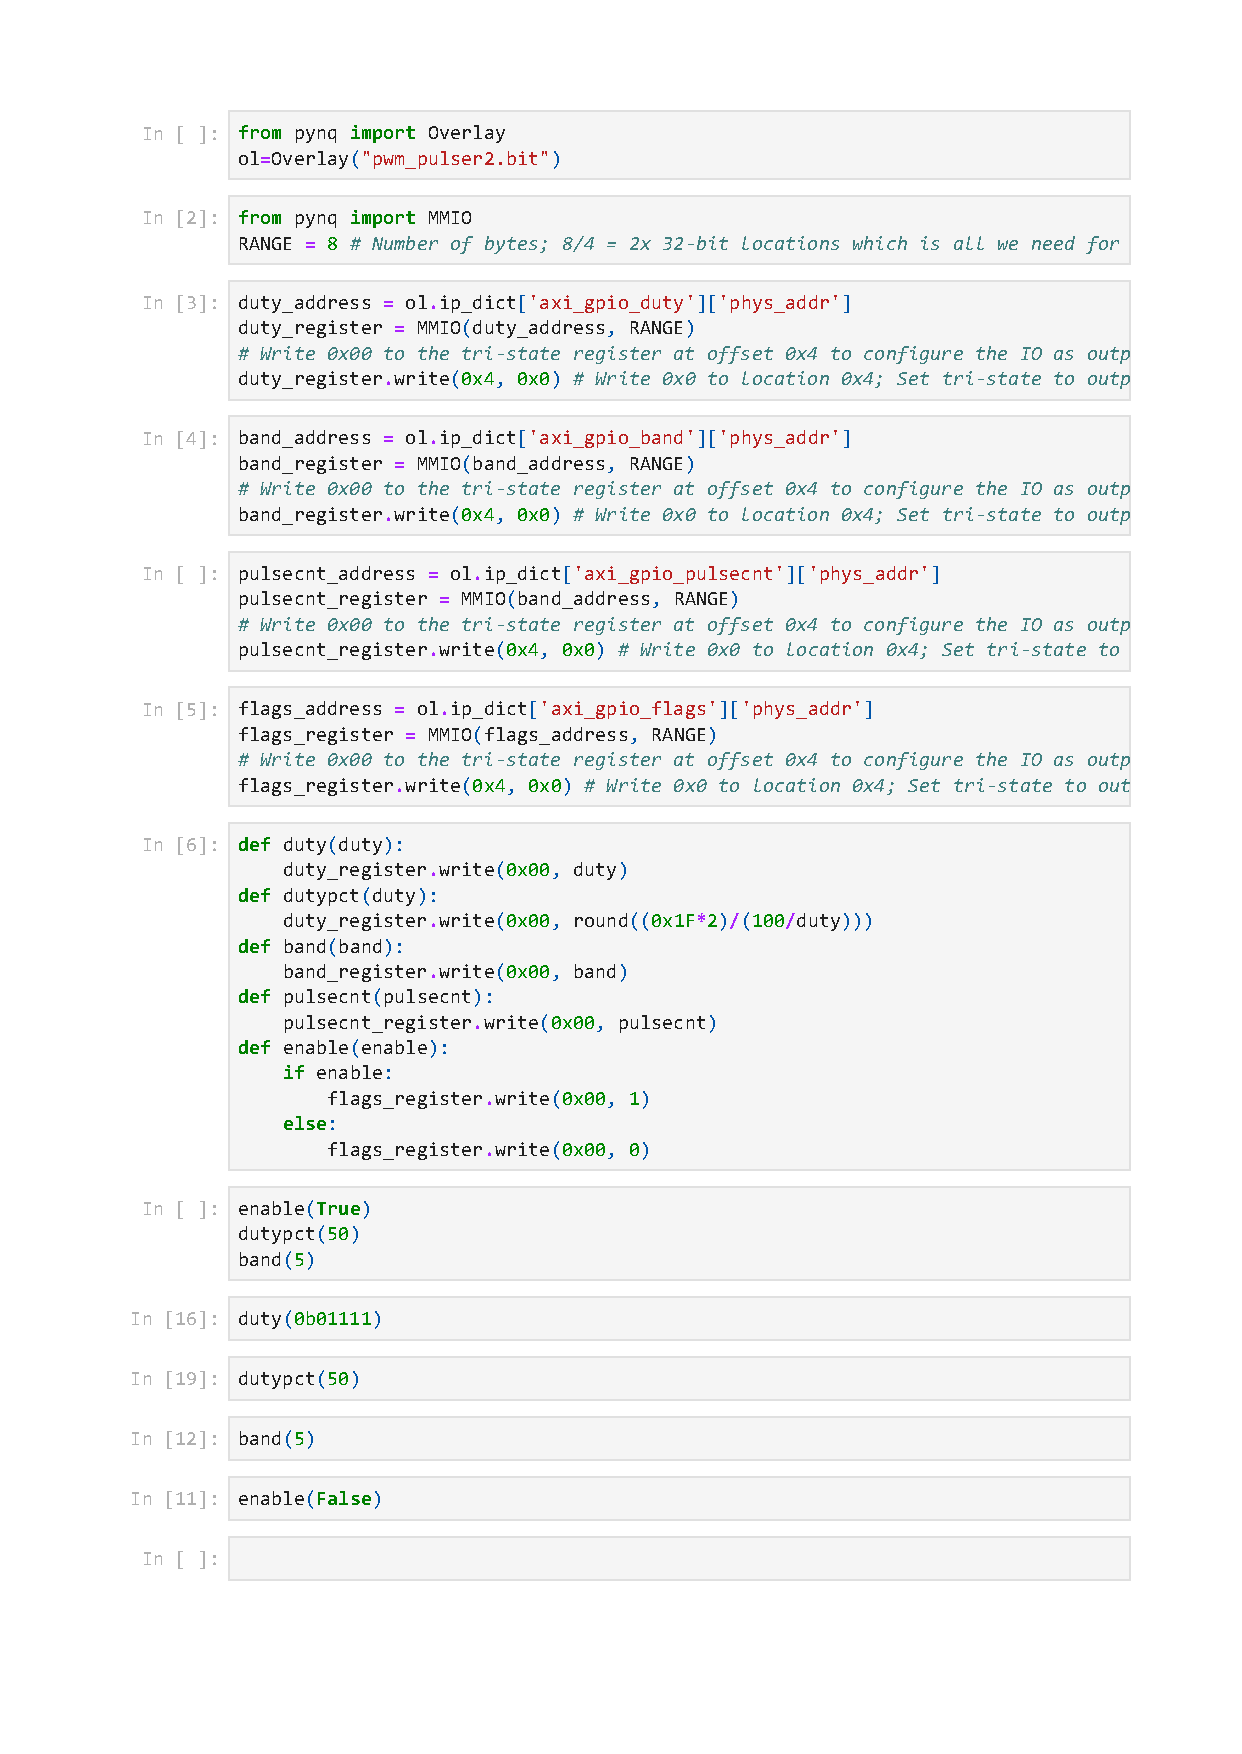
\includegraphics[height=.8\textheight]{Figures/appendix/fpga/pulser.pdf}
	\caption{Jupyter Notebook running on PYNQ Z1}
	\label{fig:app_jupyter_notebook}
\end{figure}
\begin{figure}[htbp!]
	\centering
	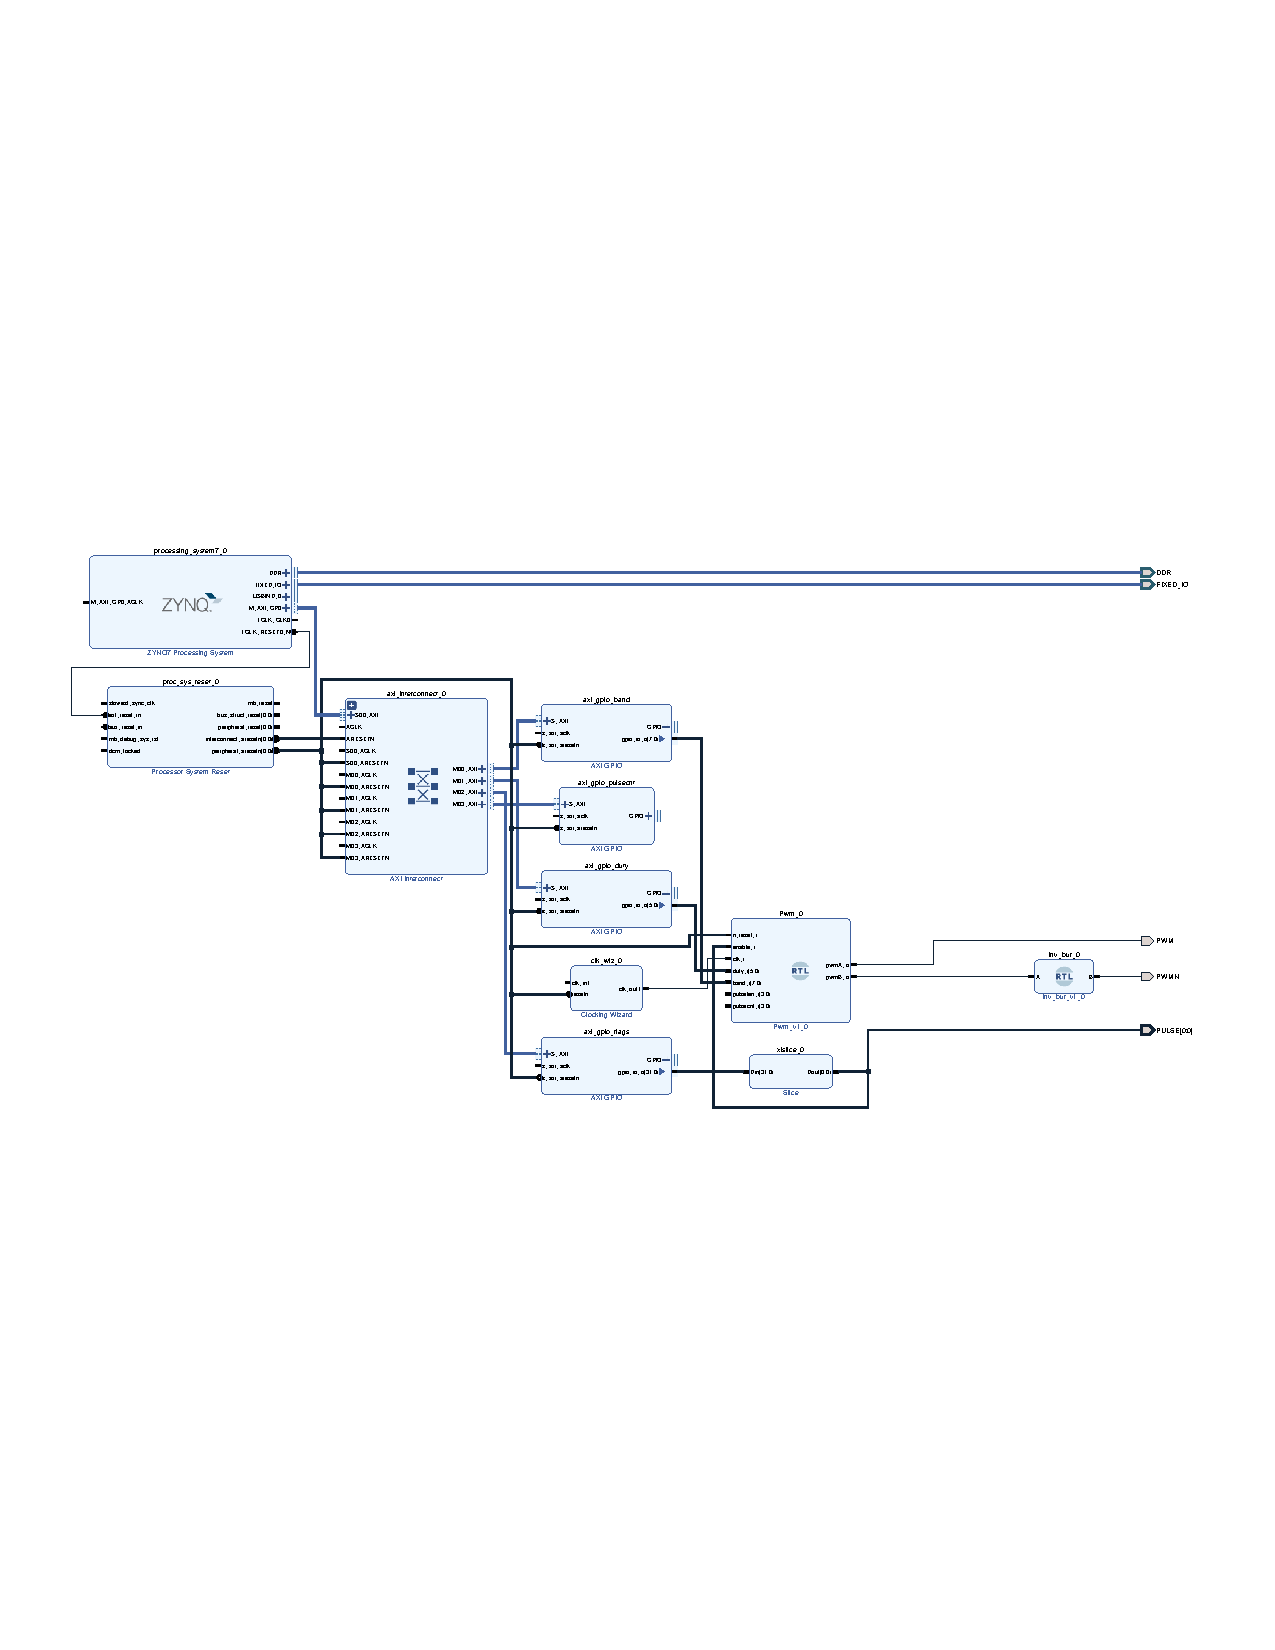
\includegraphics[width=\textwidth]{Figures/appendix/fpga/design_1.pdf}
	\caption{Block diagram of bitstream implementation}
	\label{fig:app_fpga_block_diagram}
\end{figure}
\begin{longlisting}
	\caption{Pwm.vhdl}
	\label{lst:Pwm.vhdl}
	\inputminted[bgcolor=LightGray,fontsize=\footnotesize,linenos,breaklines]{vhdl}{Figures/appendix/fpga/Pwm.vhdl}
\end{longlisting}
\begin{longlisting}
	\caption{signalcontroller.vhdl}
	\label{lst:signalcontroller.vhdl}
	\inputminted[bgcolor=LightGray,fontsize=\footnotesize,linenos,breaklines]{vhdl}{Figures/appendix/fpga/signalcontroller.vhdl}
\end{longlisting}

\section{MATLAB Scripts}
\begin{longlisting}
	\caption{US Simulation Master Script.m}
	\label{lst:sim_master}
	\inputminted[bgcolor=LightGray,fontsize=\footnotesize,linenos,breaklines]{matlab}{Figures/appendix/matlab/US_Simulation_Master_Script.m}
\end{longlisting}

\begin{longlisting}
	\caption{Analysis.m}
	\label{lst:Analysis.m}
	\inputminted[bgcolor=LightGray,fontsize=\footnotesize,linenos,breaklines]{matlab}{Figures/appendix/matlab/Analysis.m}
\end{longlisting}

\begin{longlisting}
	\caption{demodulator.m}
	\label{lst:demodulator.m}
	\inputminted[bgcolor=LightGray,fontsize=\footnotesize,linenos,breaklines]{matlab}{Figures/appendix/matlab/demodulator.m}
\end{longlisting}

\begin{longlisting}
	\caption{preamplifier.m}
	\label{lst:preamplifier.m}
	\inputminted[bgcolor=LightGray,fontsize=\footnotesize,linenos,breaklines]{matlab}{Figures/appendix/matlab/preamplifier.m}
\end{longlisting}

\begin{longlisting}
	\caption{sampler.m}
	\label{lst:sampler.m}
	\inputminted[bgcolor=LightGray,fontsize=\footnotesize,linenos,breaklines]{matlab}{Figures/appendix/matlab/sampler.m}
\end{longlisting}

\begin{longlisting}
	\caption{transmitter.m}
	\label{lst:transmitter.m}
	\inputminted[bgcolor=LightGray,fontsize=\footnotesize,linenos,breaklines]{matlab}{Figures/appendix/matlab/transmitter.m}
\end{longlisting}

\begin{longlisting}
	\caption{vna.m}
	\label{lst:vna.m}
	\inputminted[bgcolor=LightGray,fontsize=\footnotesize,linenos,breaklines]{matlab}{Figures/appendix/matlab/vna.m}
\end{longlisting}

\begin{longlisting}
	\caption{bpf datasheet s21.m}
	\label{lst:bpf_datasheet_s21.m}
	\inputminted[bgcolor=LightGray,fontsize=\footnotesize,linenos,breaklines]{matlab}{Figures/appendix/matlab/datasheet_s21.m}
\end{longlisting}

\begin{longlisting}
	\caption{switch.m}
	\label{lst:switch.m}
	\inputminted[bgcolor=LightGray,fontsize=\footnotesize,linenos,breaklines]{matlab}{Figures/appendix/matlab/Switch_demo.m}
\end{longlisting}


\chapter{Simulation Models}
\begin{figure}[htbp]
	\centering
	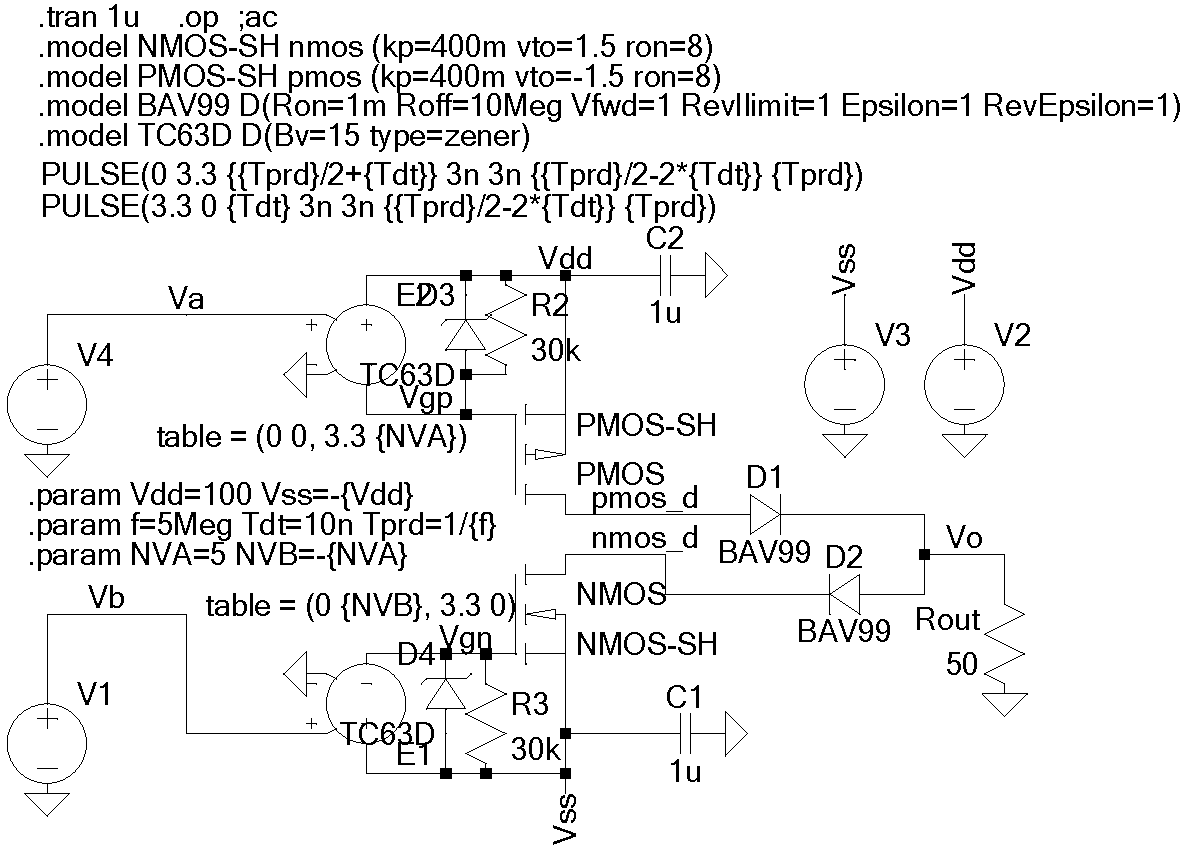
\includegraphics[width=.9\textwidth]{Figures/appendix/ltspice_transmitter.pdf}
	\caption{LTspice model of transmitter}
	\label{fig:app_ltspice_transmitter}
\end{figure}
\begin{figure}[htbp]
	\centering
	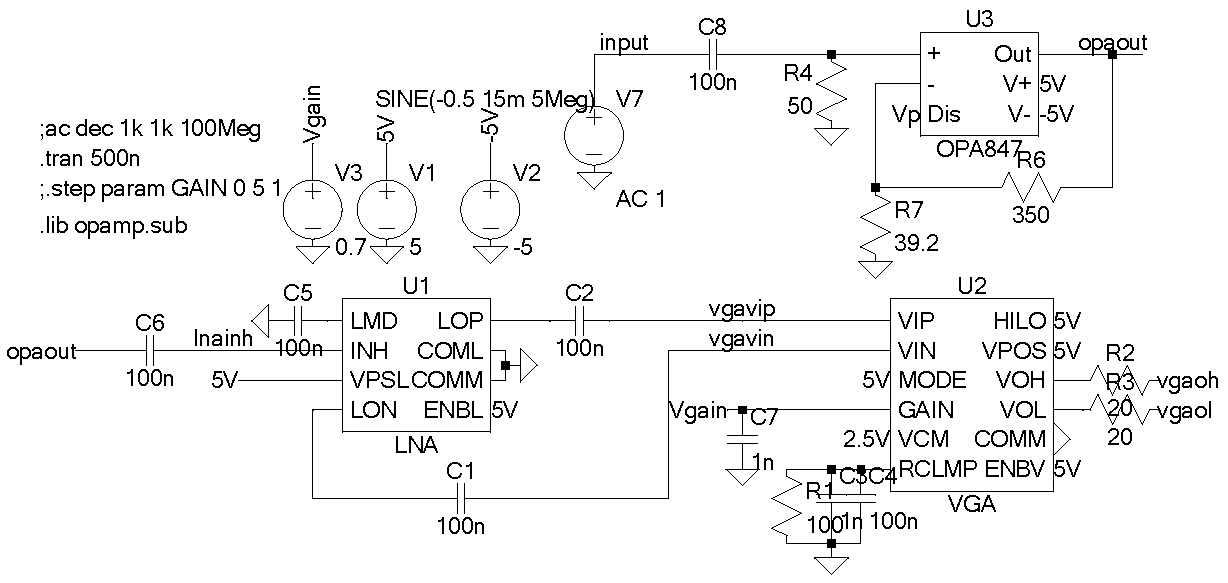
\includegraphics[width=.9\textwidth]{Figures/appendix/ltspice_preamp.pdf}
	\caption{LTspice model of preamplifier}
	\label{fig:app_ltspice_preamp}
\end{figure}
\begin{figure}[htbp]
	\centering
	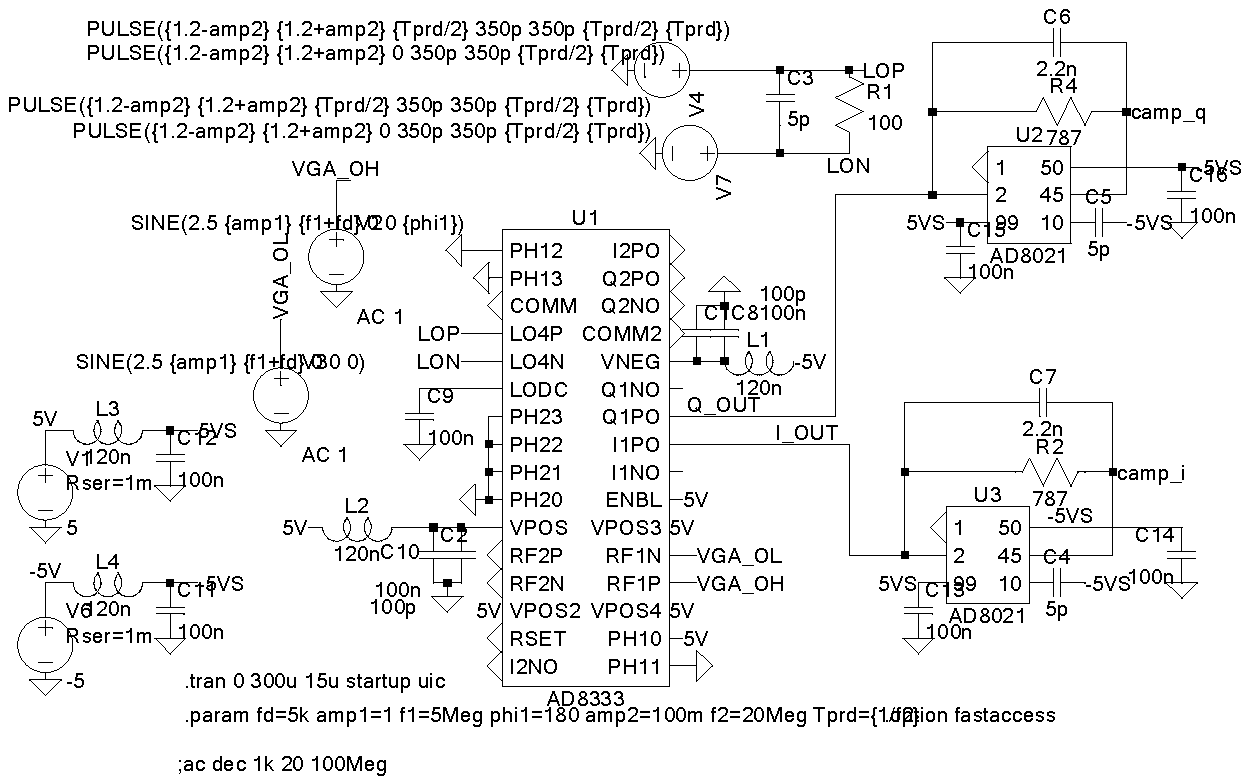
\includegraphics[width=.9\textwidth]{Figures/appendix/ltspice_demod.pdf}
	\caption{LTspice model of demodulator}
	\label{fig:app_ltspice_demod}
\end{figure}
\begin{figure}[htbp]
	\centering
	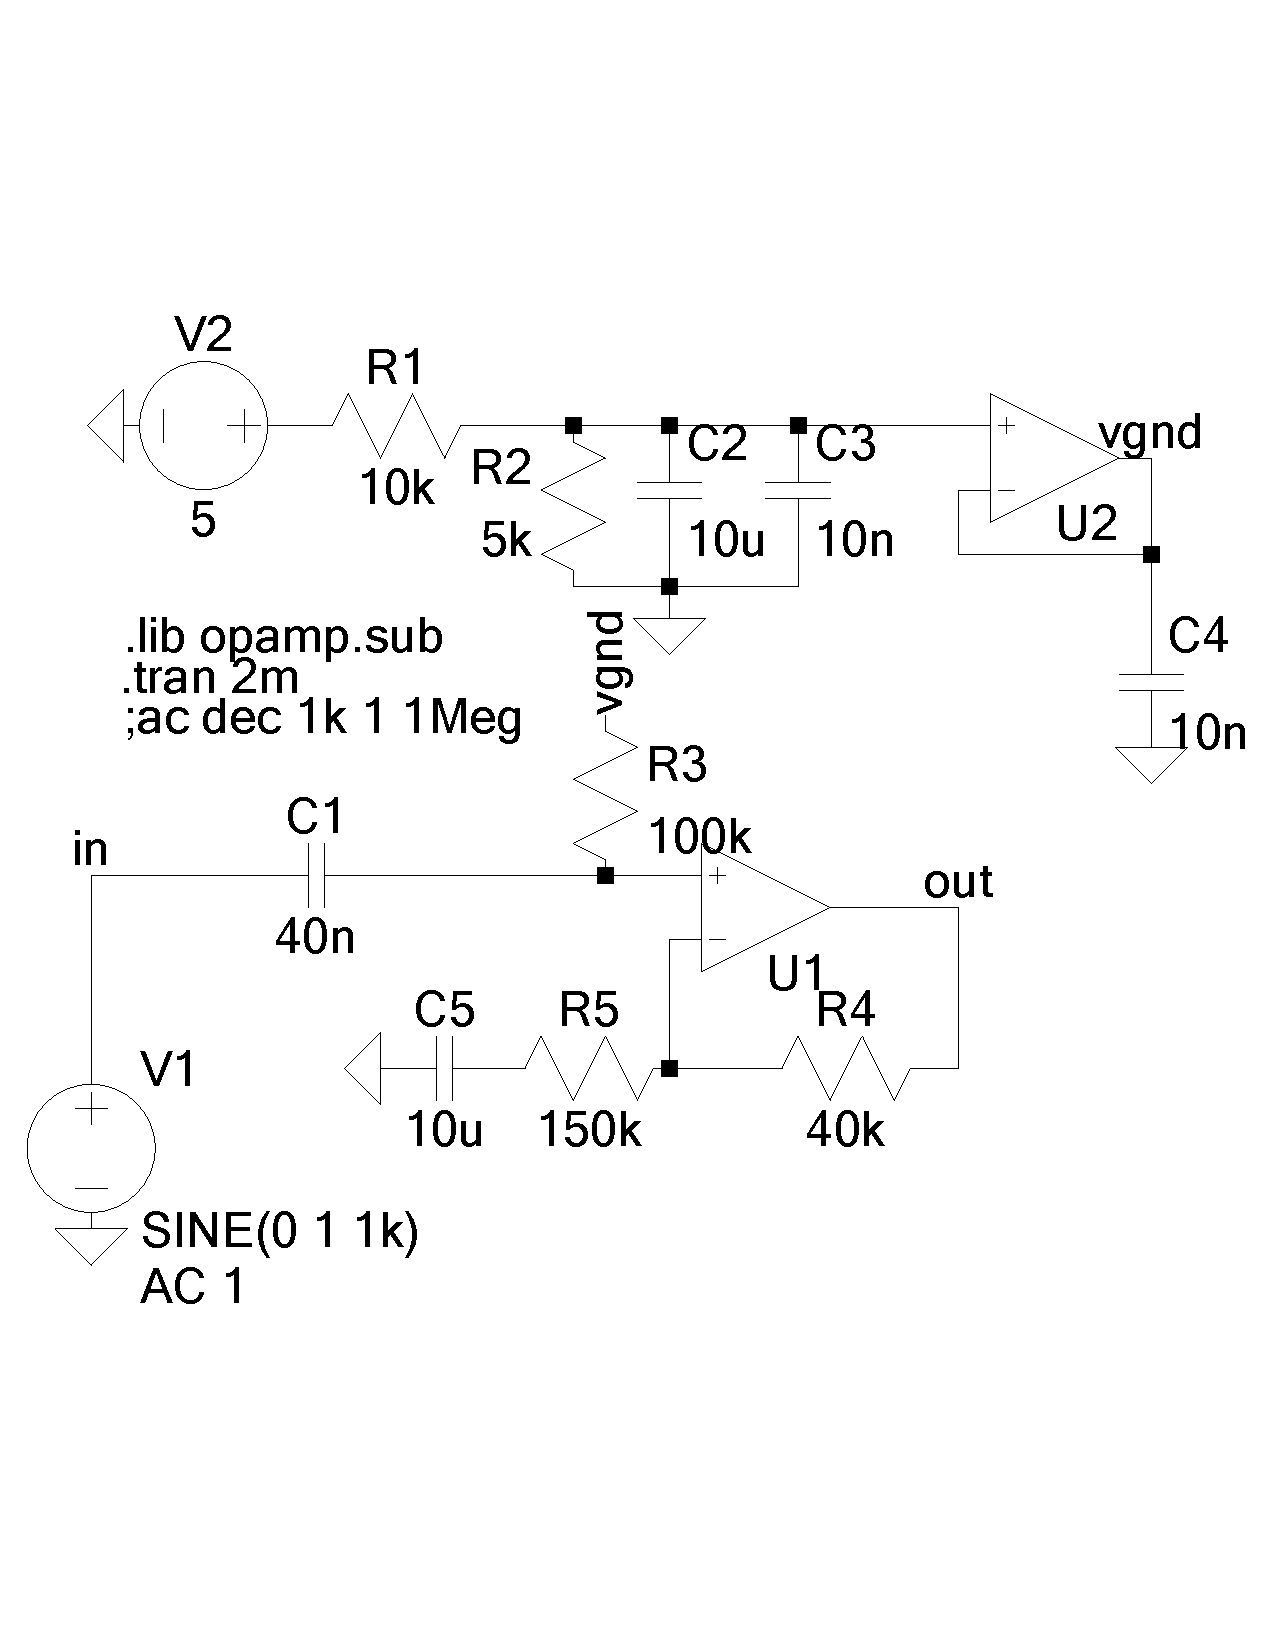
\includegraphics[width=.9\textwidth]{Figures/appendix/ltspice_dccoupler.pdf}
	\caption{LTspice model of PRF filter}
	\label{fig:app_ltspice_dc_coupler}
\end{figure}


%\chapter{Timer Configurations}
%\begin{figure}[htbp]
%	\centering
%	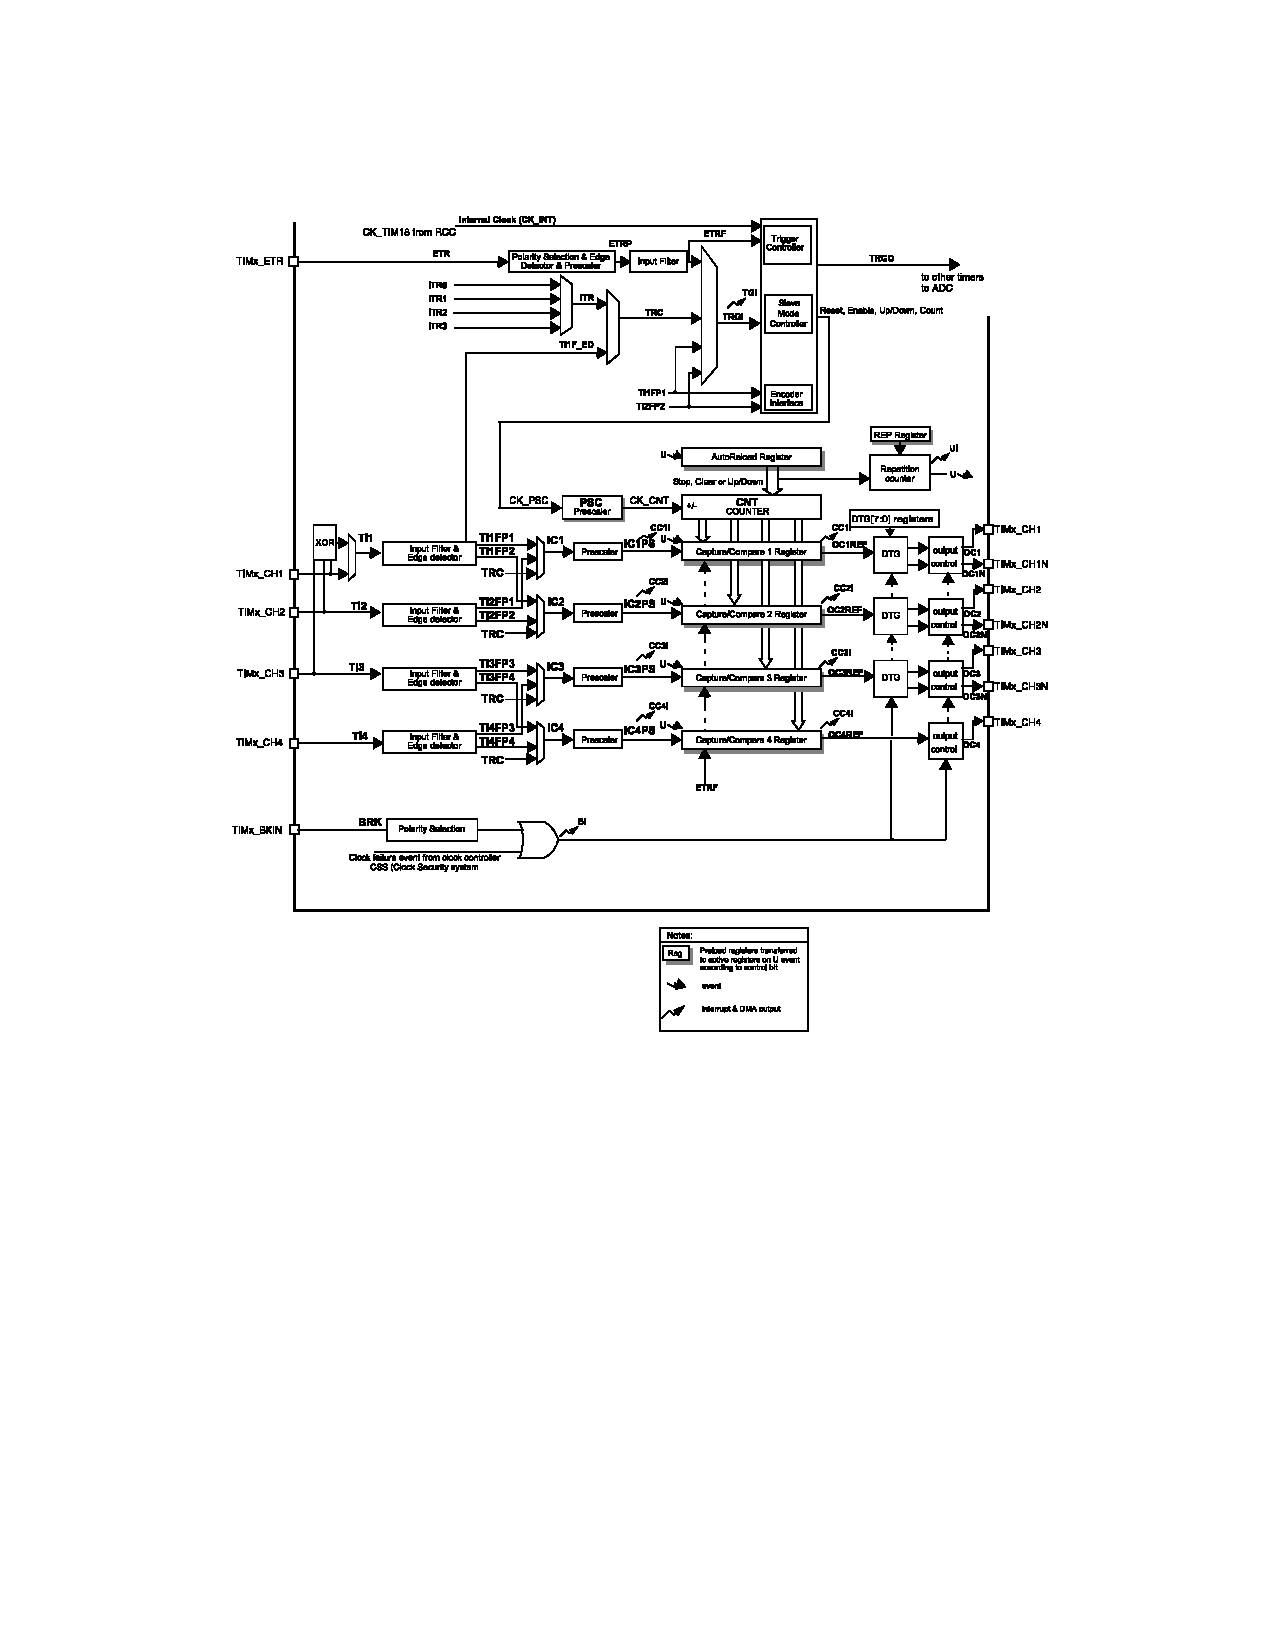
\includegraphics[width=.8\textwidth]{Figures/4_advanced_timer1_diagram.pdf}
%	\caption{Configuration of \texttt{TIMER1}}
%	\label{fig:4_timer1}
%\end{figure}
%\begin{figure}[htbp]
%	\centering
%	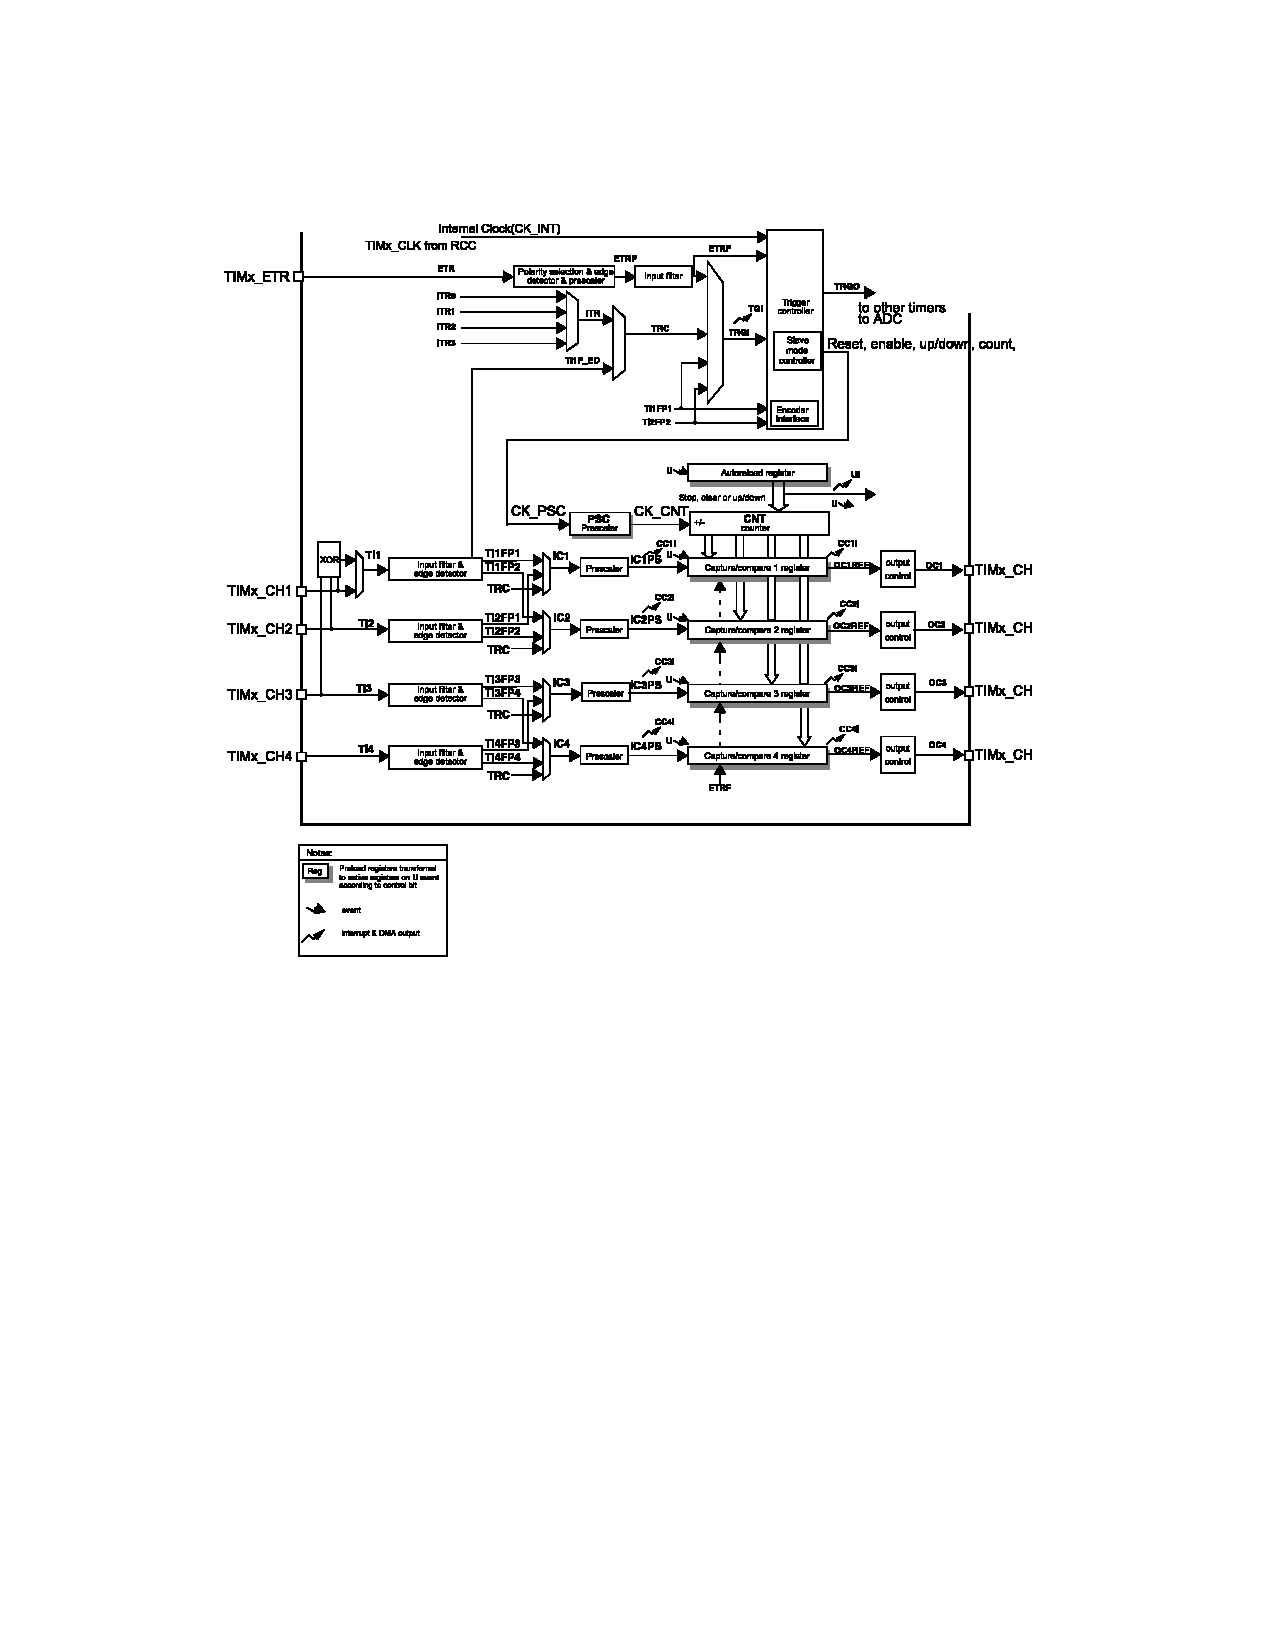
\includegraphics[width=.8\textwidth]{Figures/4_advanced_timer2-5_diagram.pdf}
%	\caption{Configuration of \texttt{TIMER2--5}}
%	\label{fig:4_timer2-5}
%\end{figure}
%\begin{figure}[htbp]
%	\centering
%	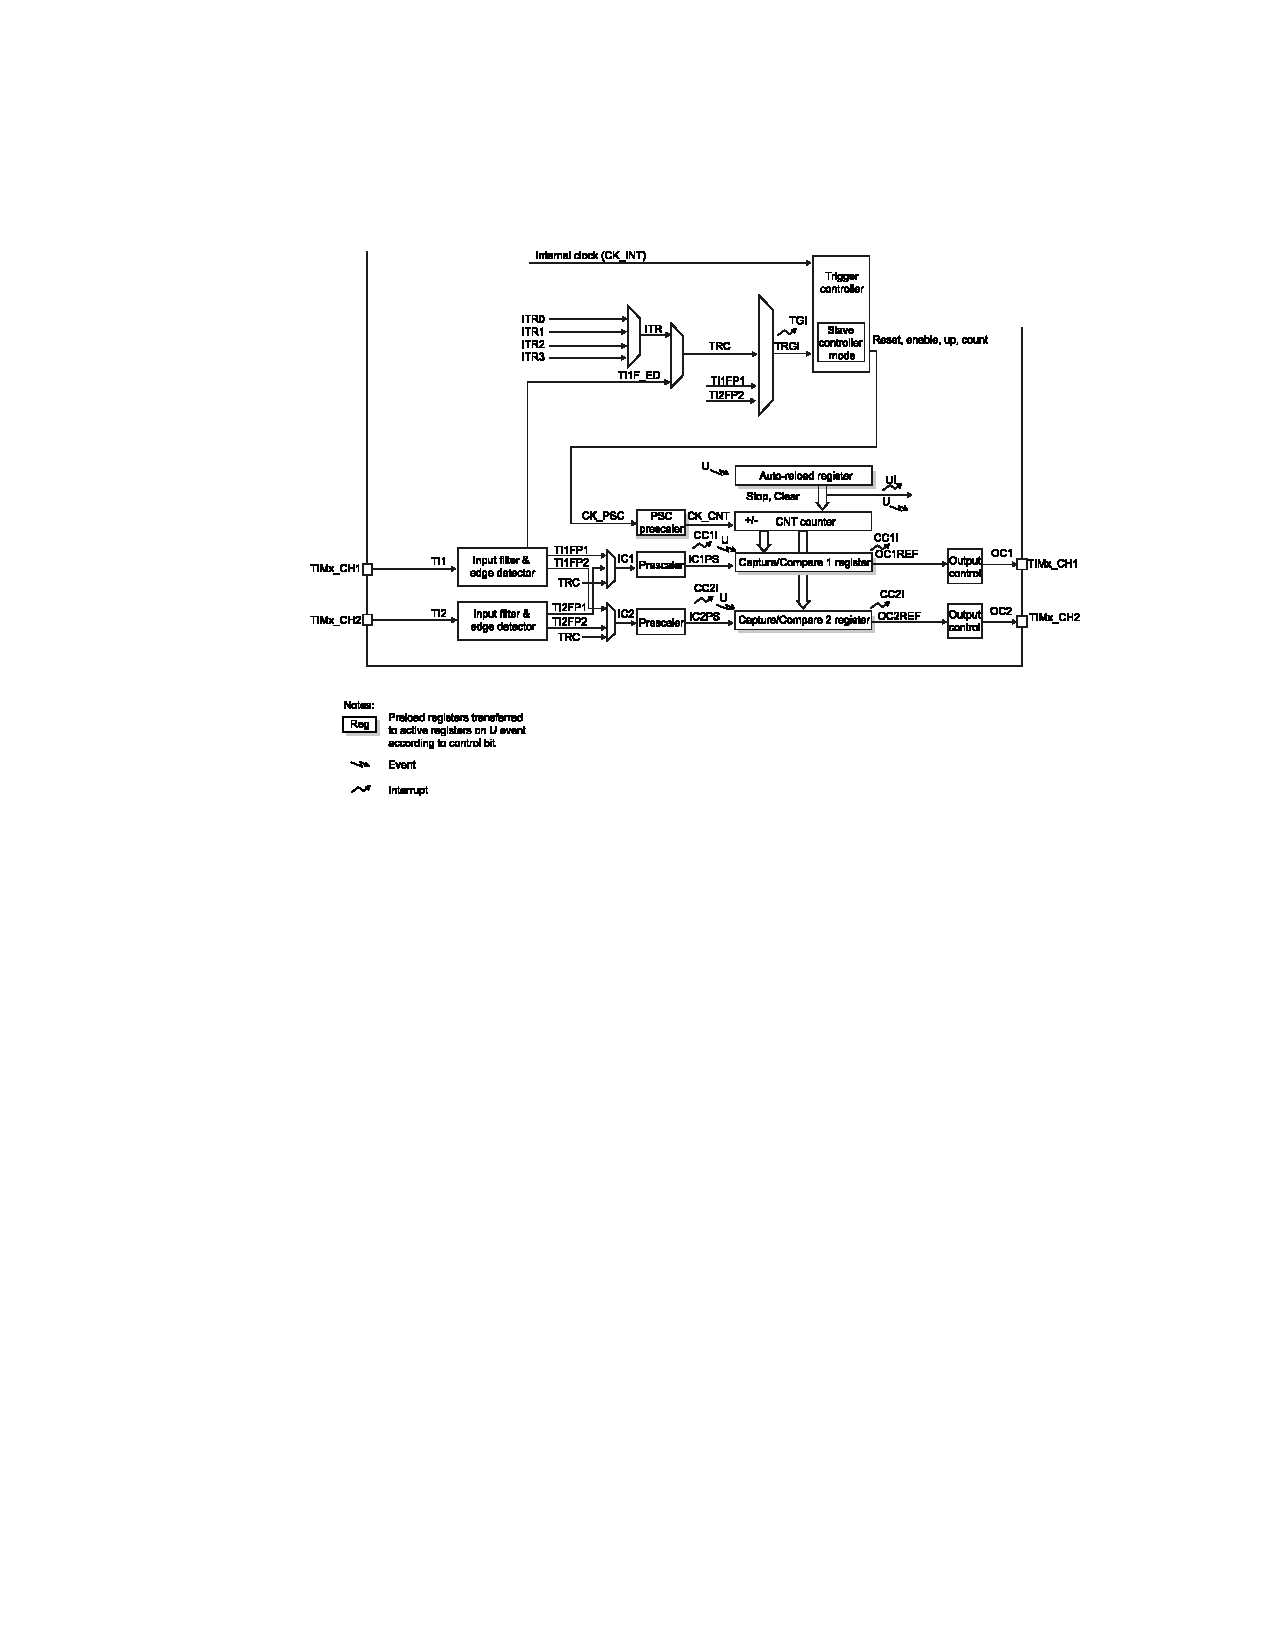
\includegraphics[width=.8\textwidth]{Figures/4_advanced_timer9_diagram.pdf}
%	\caption{Configuration of \texttt{TIMER9}}
%	\label{fig:4_timer9}
%\end{figure}


\chapter{Circuit Schematics}
\begin{landscape}
	\begin{figure}[htbp]
		\centering
		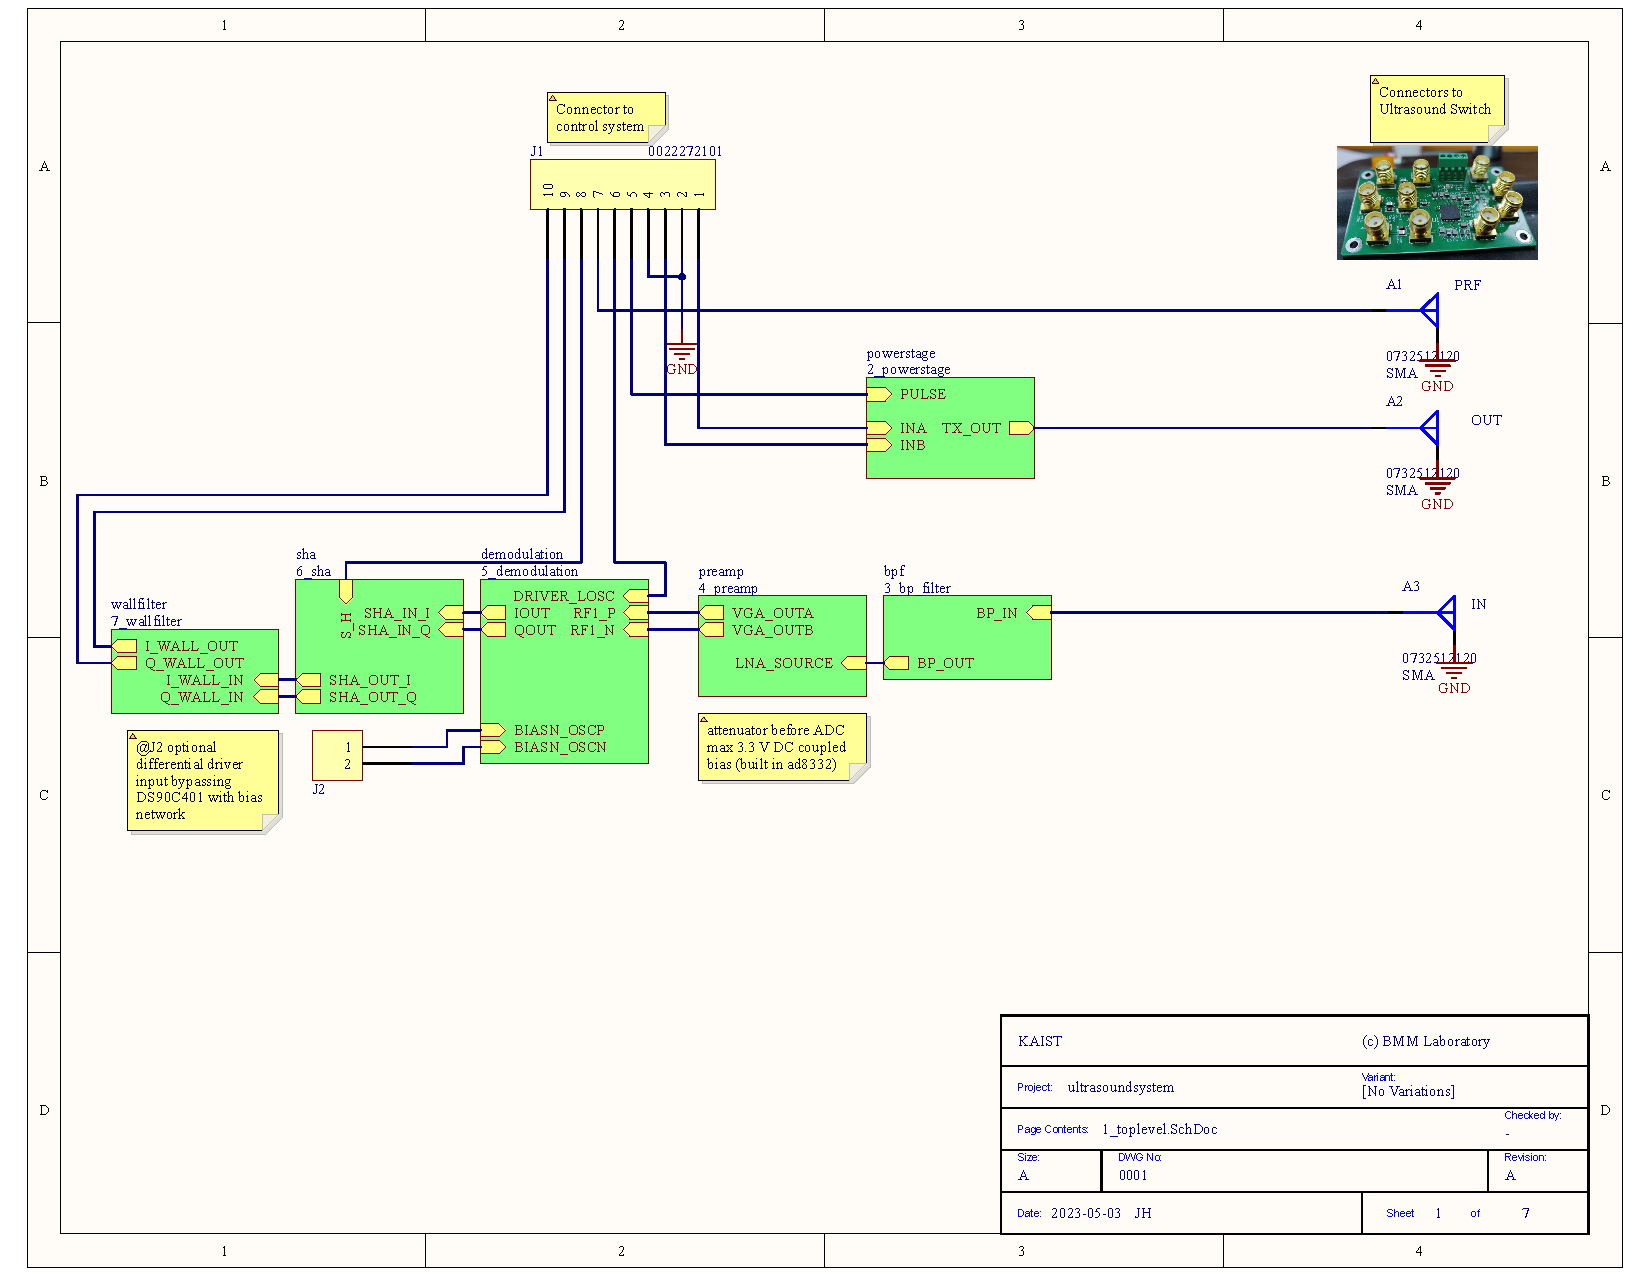
\includegraphics[width=20cm,height=28.7cm,keepaspectratio]{Figures/appendix/afe_altium/1_toplevel.pdf}
		\caption{AFE Top Level}
		\label{fig:appendix_1_toplevel}
	\end{figure}
\end{landscape}
\begin{landscape}
	\begin{figure}[htbp]
		\centering
		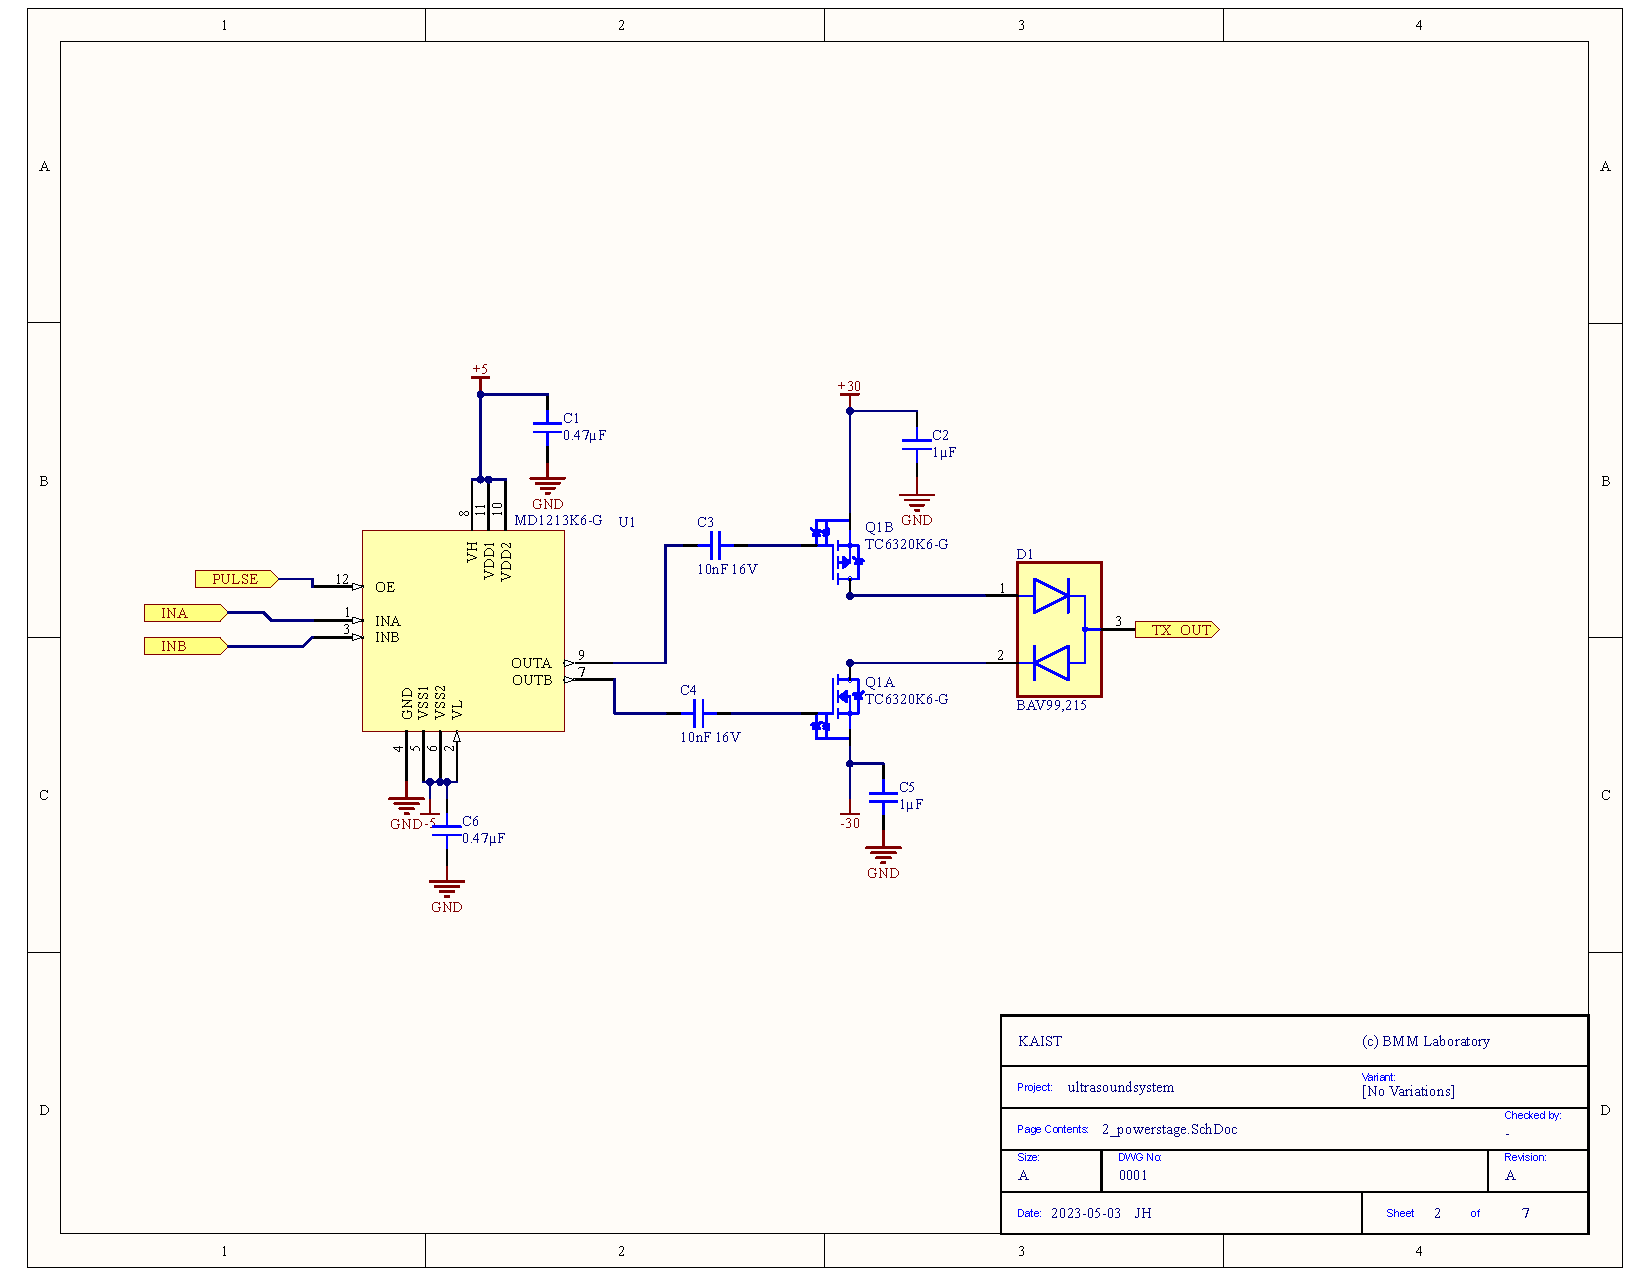
\includegraphics[width=20cm,height=28.7cm,keepaspectratio]{Figures/appendix/afe_altium/2_powerstage.pdf}
		\caption{AFE Power Stage}
		\label{fig:appendix_2_powerstage}
	\end{figure}
\end{landscape}
\begin{landscape}
	\begin{figure}[htbp]
		\centering
		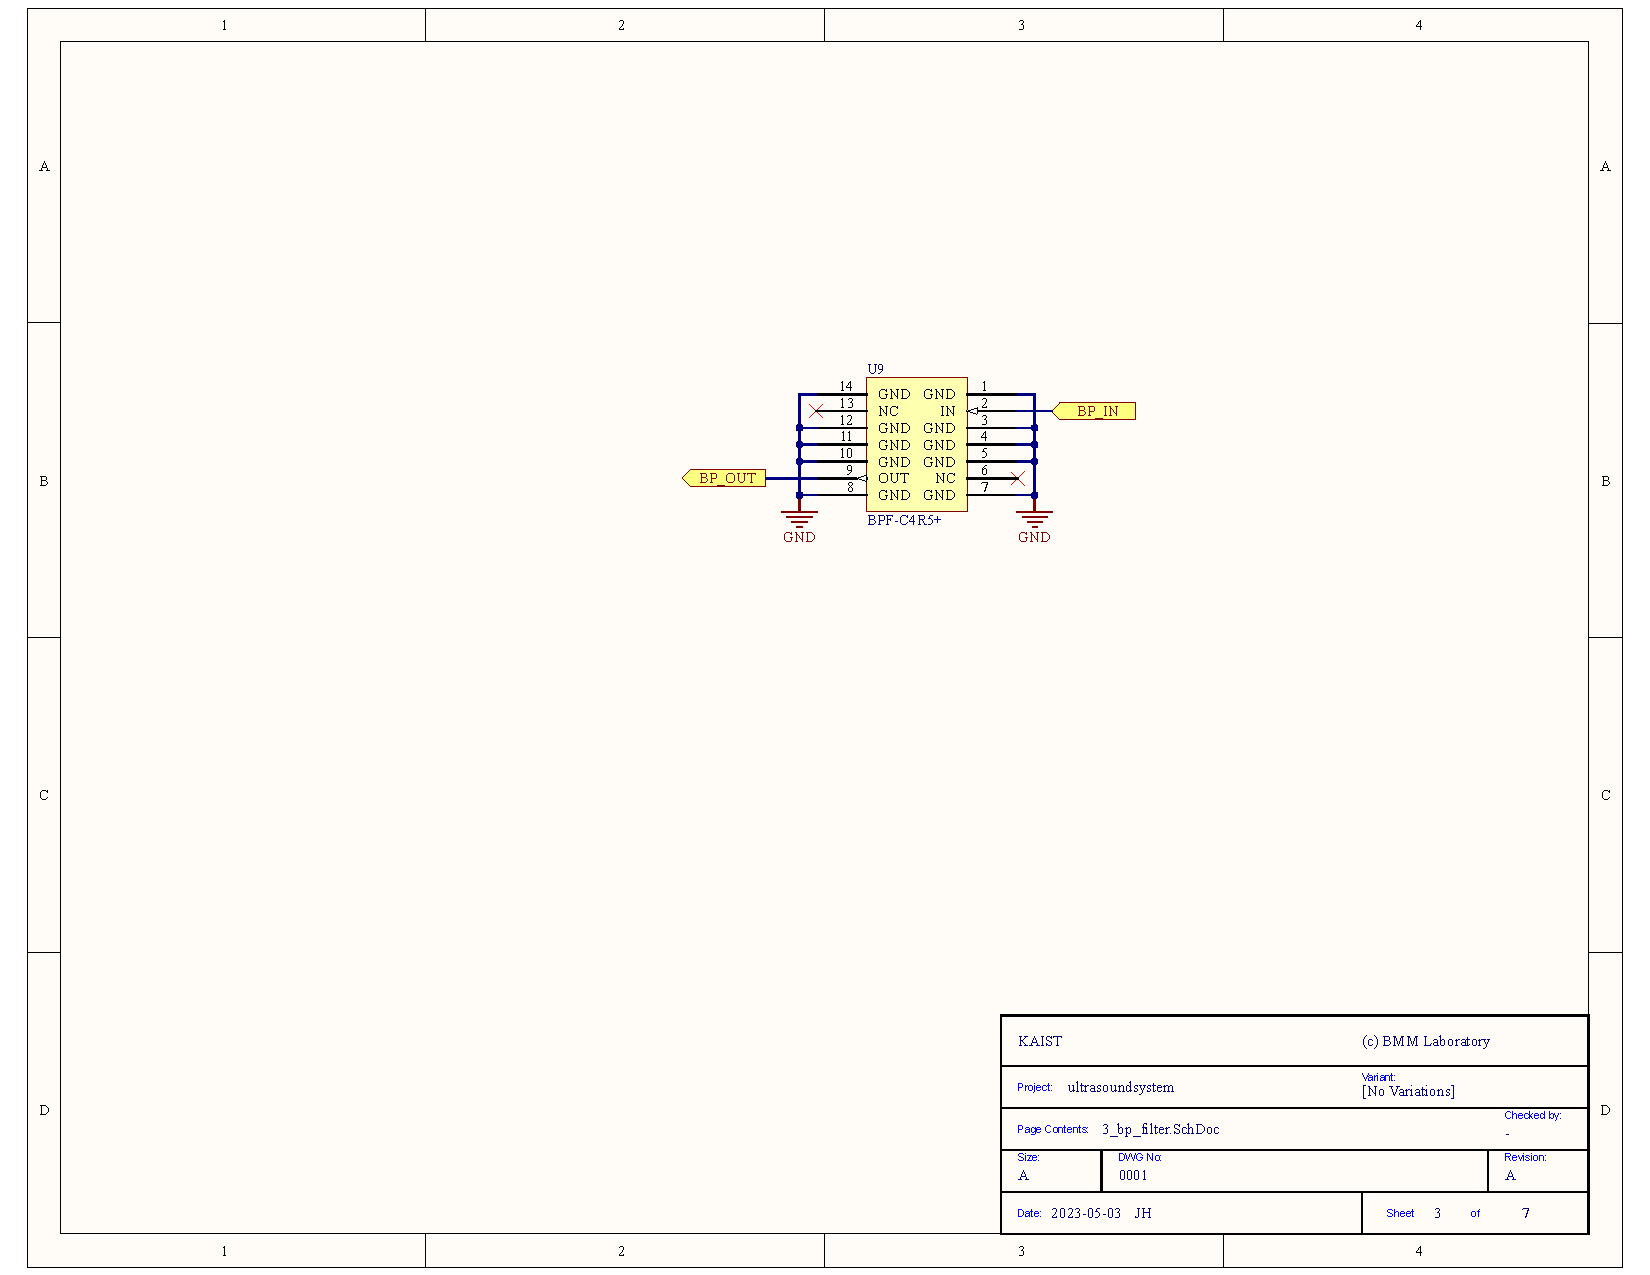
\includegraphics[width=20cm,height=28.7cm,keepaspectratio]{Figures/appendix/afe_altium/3_bpf.pdf}
		\caption{AFE BPF}
		\label{fig:appendix_3_bpf}
	\end{figure}
\end{landscape}
\begin{landscape}
	\begin{figure}[htbp]
		\centering
		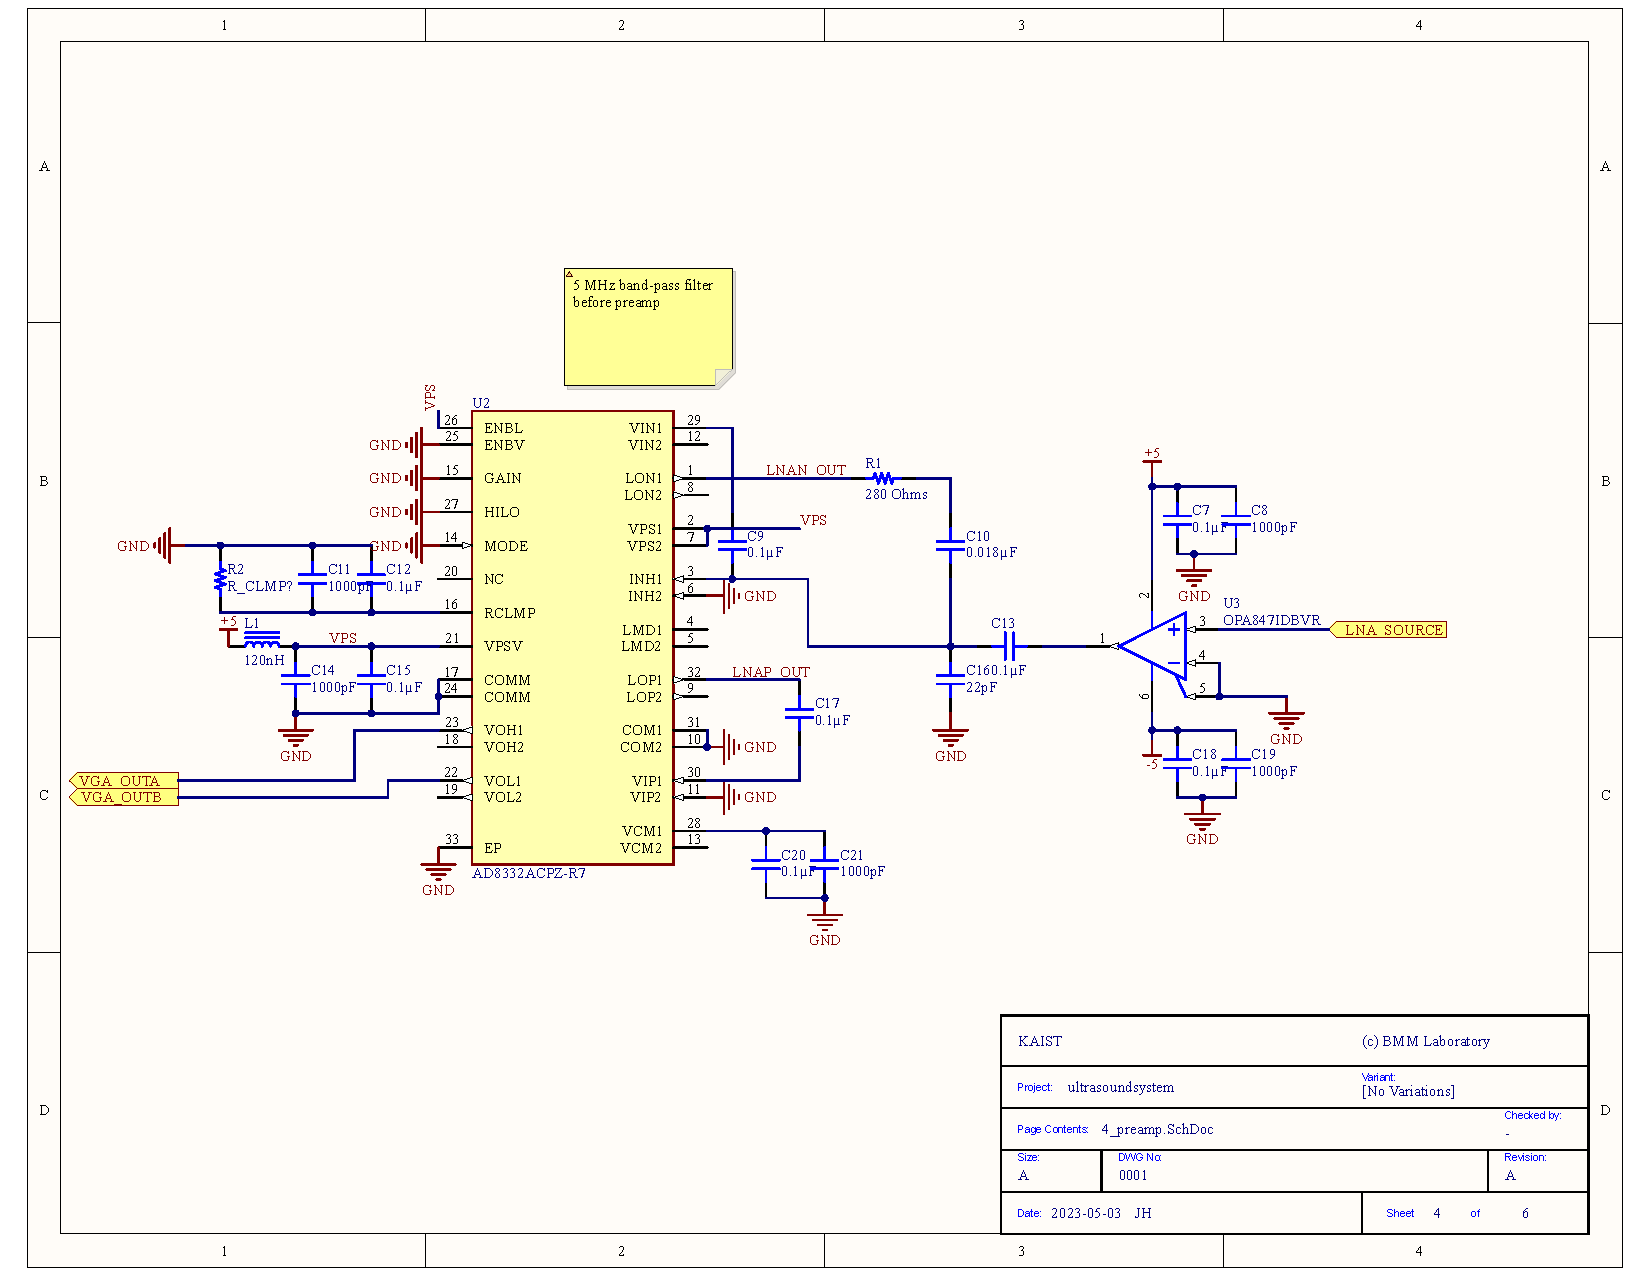
\includegraphics[width=20cm,height=28.7cm,keepaspectratio]{Figures/appendix/afe_altium/4_preamp.pdf}
		\caption{AFE Preamplifier}
		\label{fig:appendix_4_preamp}
	\end{figure}
\end{landscape}
\begin{landscape}
	\begin{figure}[htbp]
		\centering
		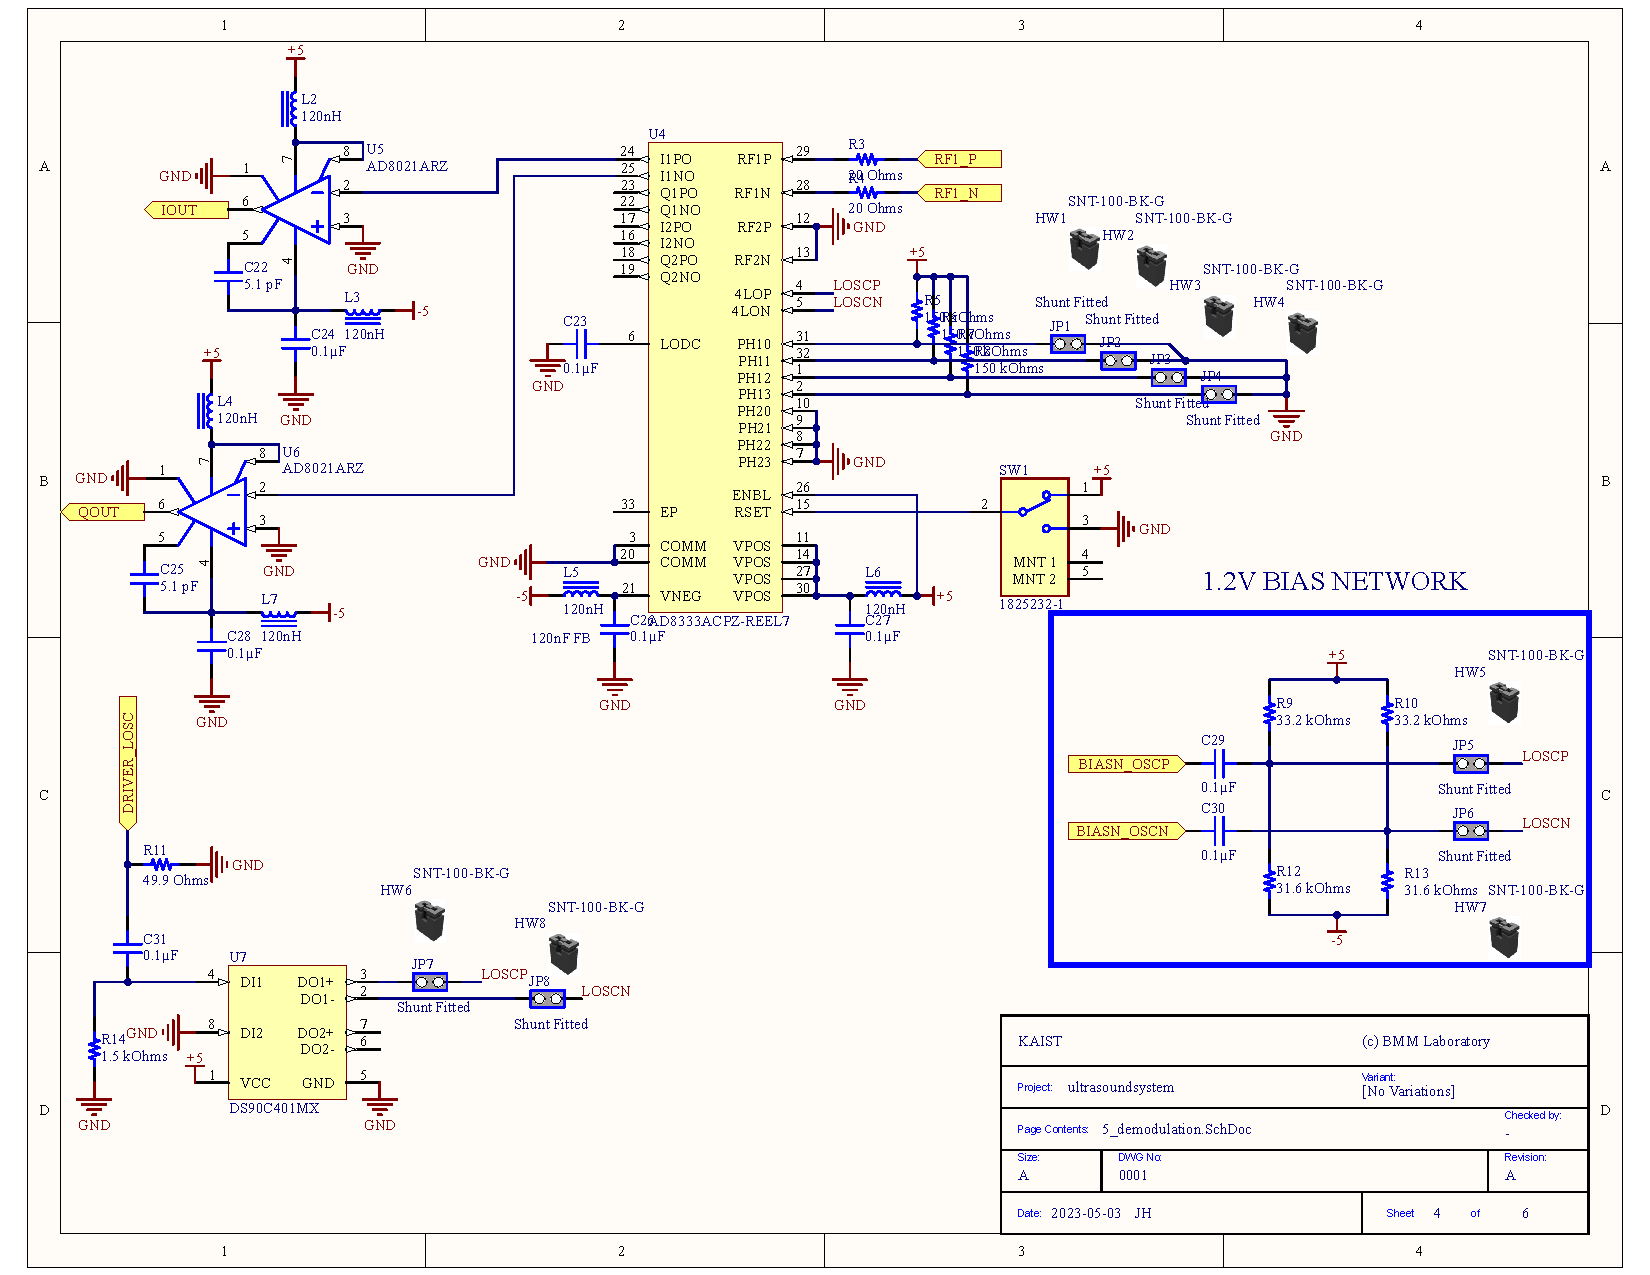
\includegraphics[width=20cm,height=28.7cm,keepaspectratio]{Figures/appendix/afe_altium/5_demodulator.pdf}
		\caption{AFE Demodulator}
		\label{fig:appendix_5_demodulator}
	\end{figure}
\end{landscape}
\begin{landscape}
	\begin{figure}[htbp]
		\centering
		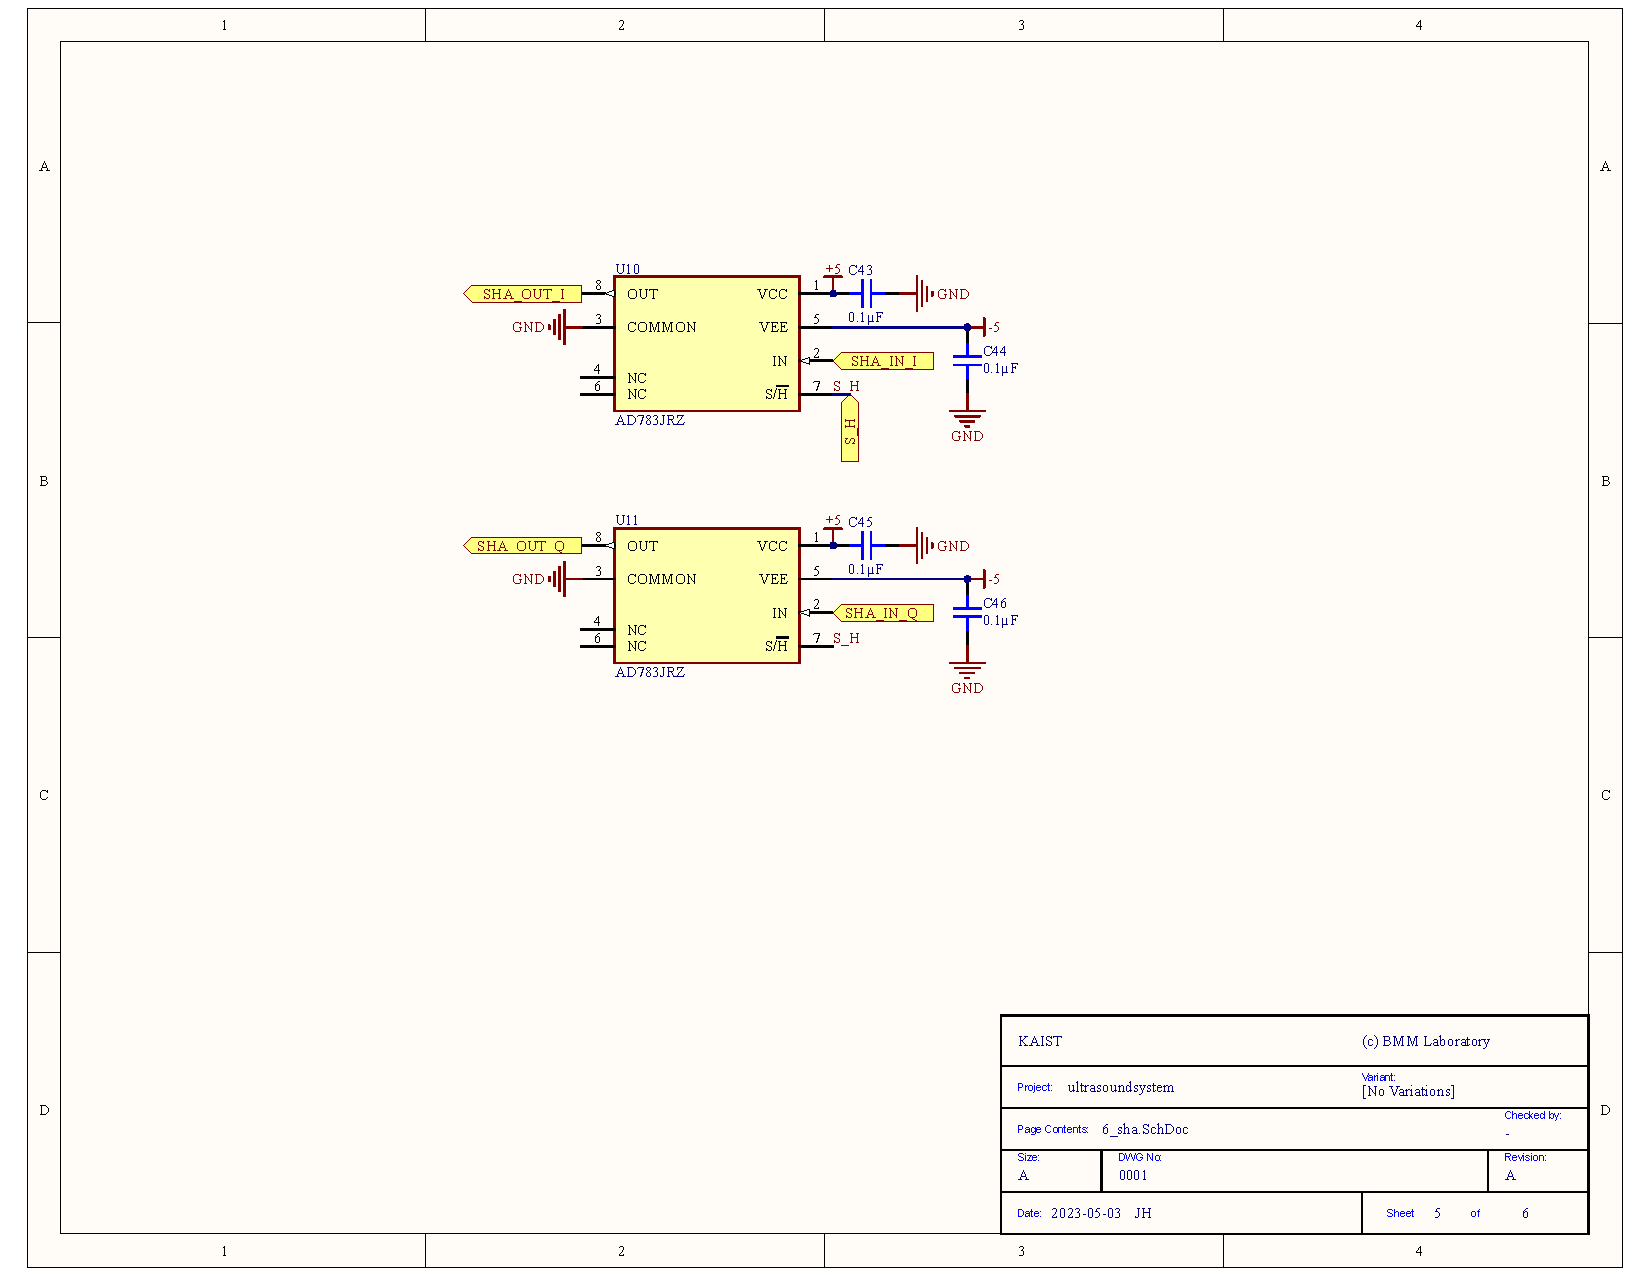
\includegraphics[width=20cm,height=28.7cm,keepaspectratio]{Figures/appendix/afe_altium/6_sha.pdf}
		\caption{AFE Sample and Hold Amplifier}
		\label{fig:appendix_6_sha}
	\end{figure}
\end{landscape}
\begin{landscape}
	\begin{figure}[htbp]
		\centering
		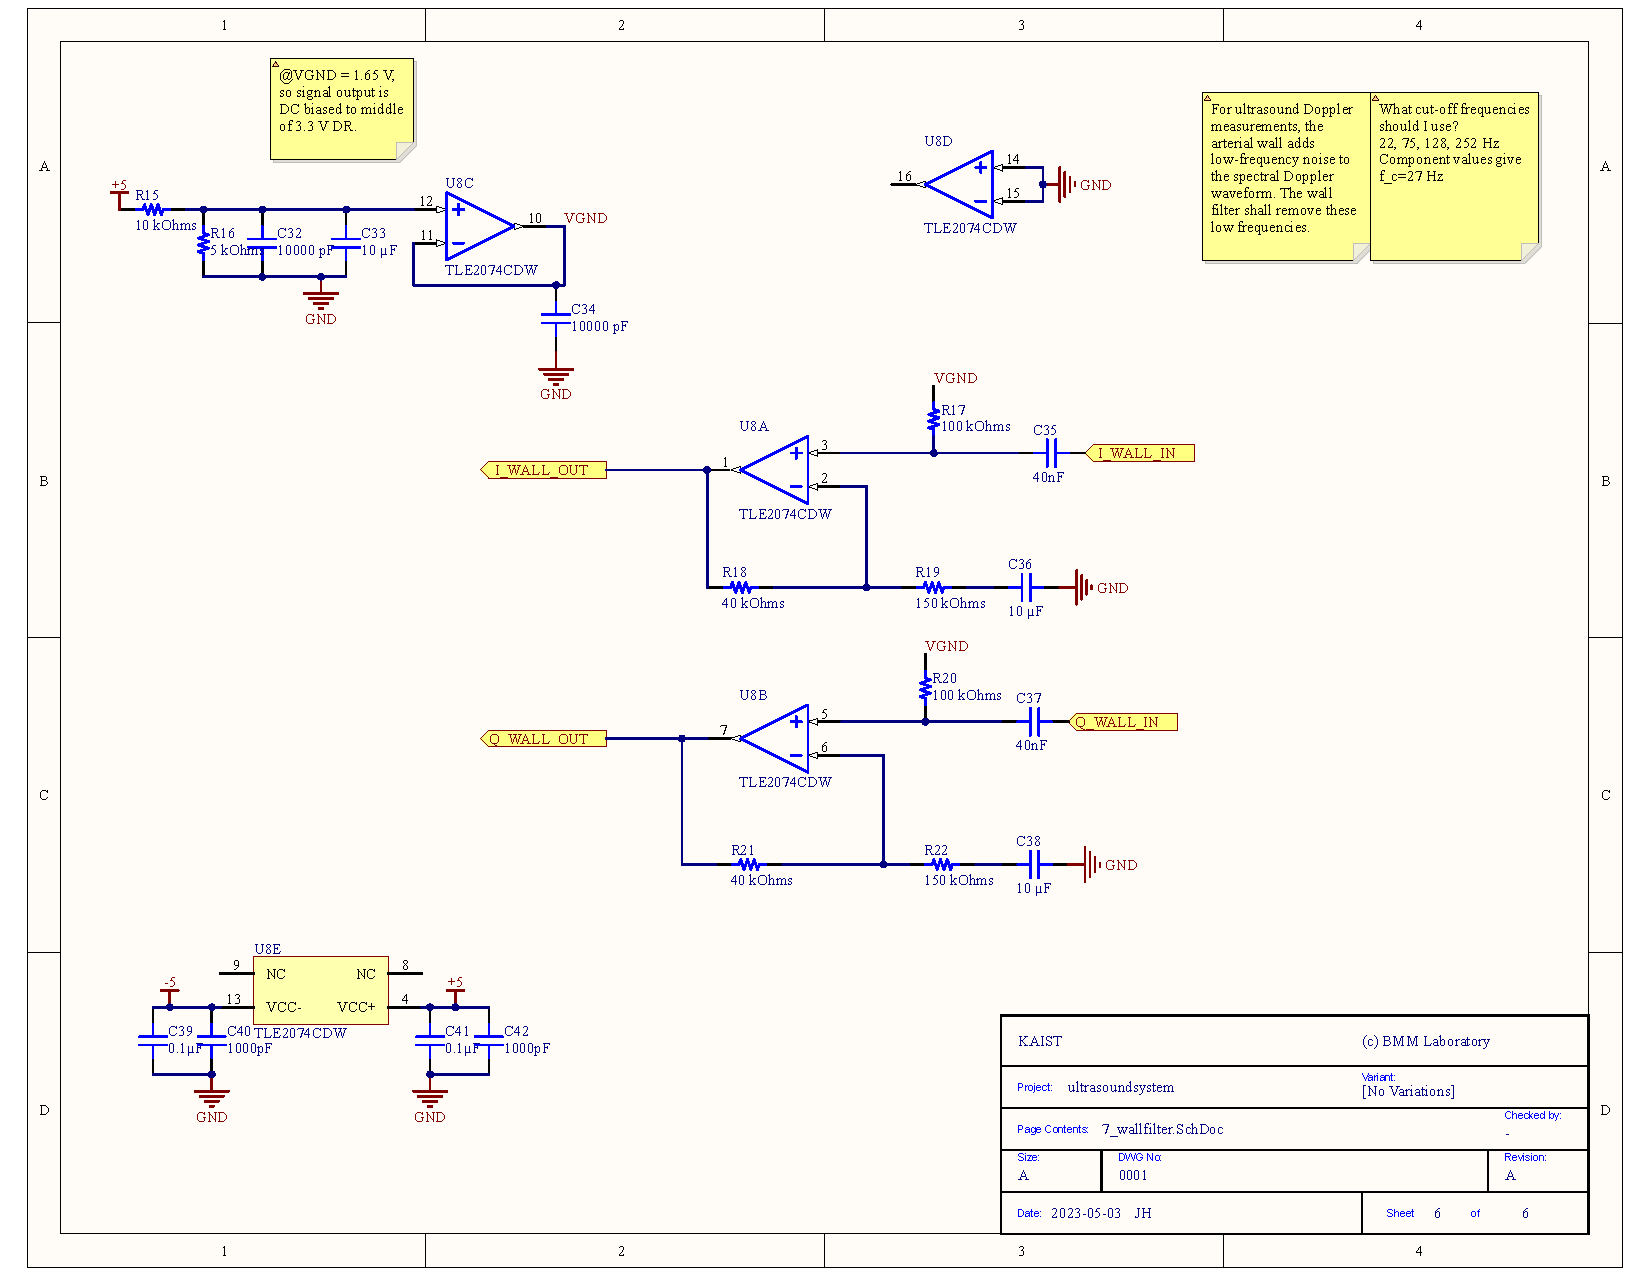
\includegraphics[width=20cm,height=28.7cm,keepaspectratio]{Figures/appendix/afe_altium/7_wallfilter.pdf}
		\caption{AFE Wall Filter}
		\label{fig:appendix_7_wallfilter}
	\end{figure}
\end{landscape}
\begin{landscape}
	\begin{figure}[htbp]
		\centering
		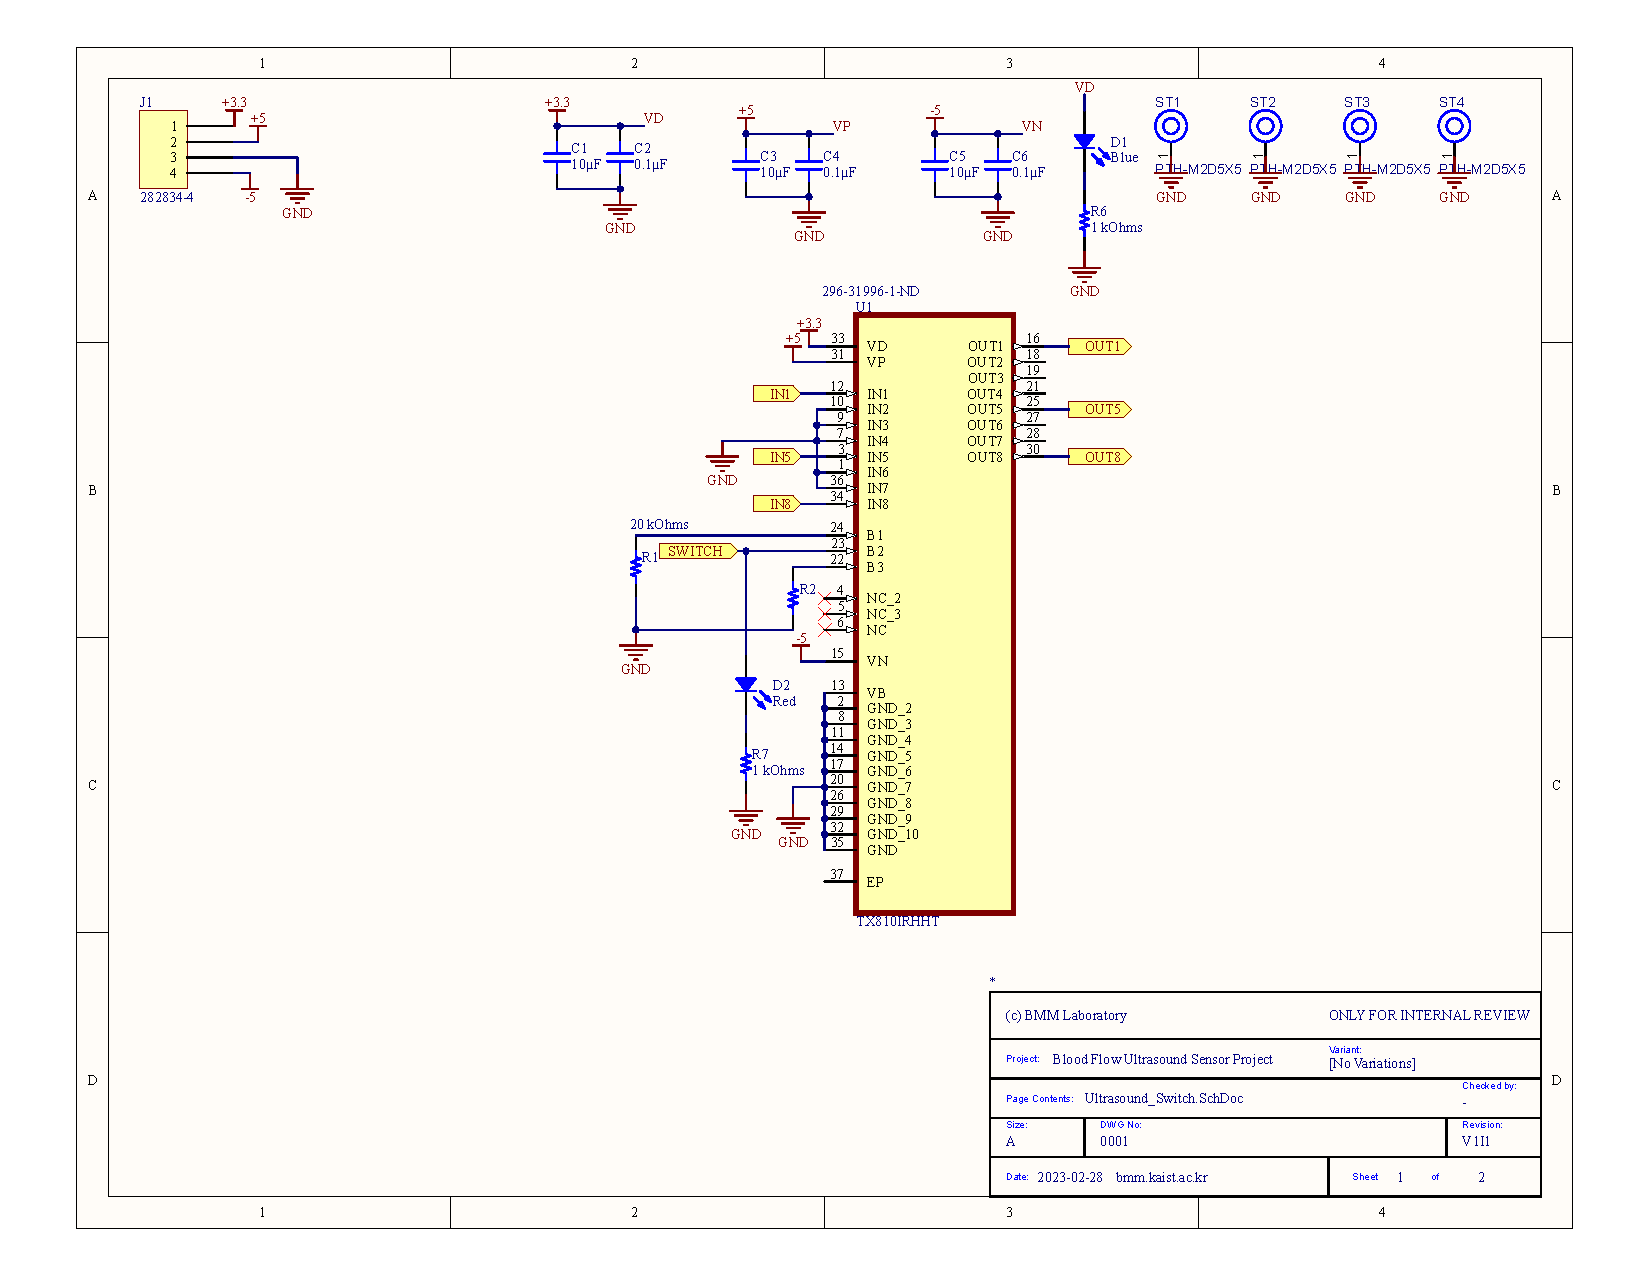
\includegraphics[width=20cm,height=28.7cm,keepaspectratio]{Figures/appendix/ultrasound_switch.pdf}
		\caption{UltrasoundSwitch Schematic A}
		\label{fig:appendix_ultrasoundswitch_a}
	\end{figure}
\end{landscape}
\begin{landscape}
	\begin{figure}[htbp]
		\centering
		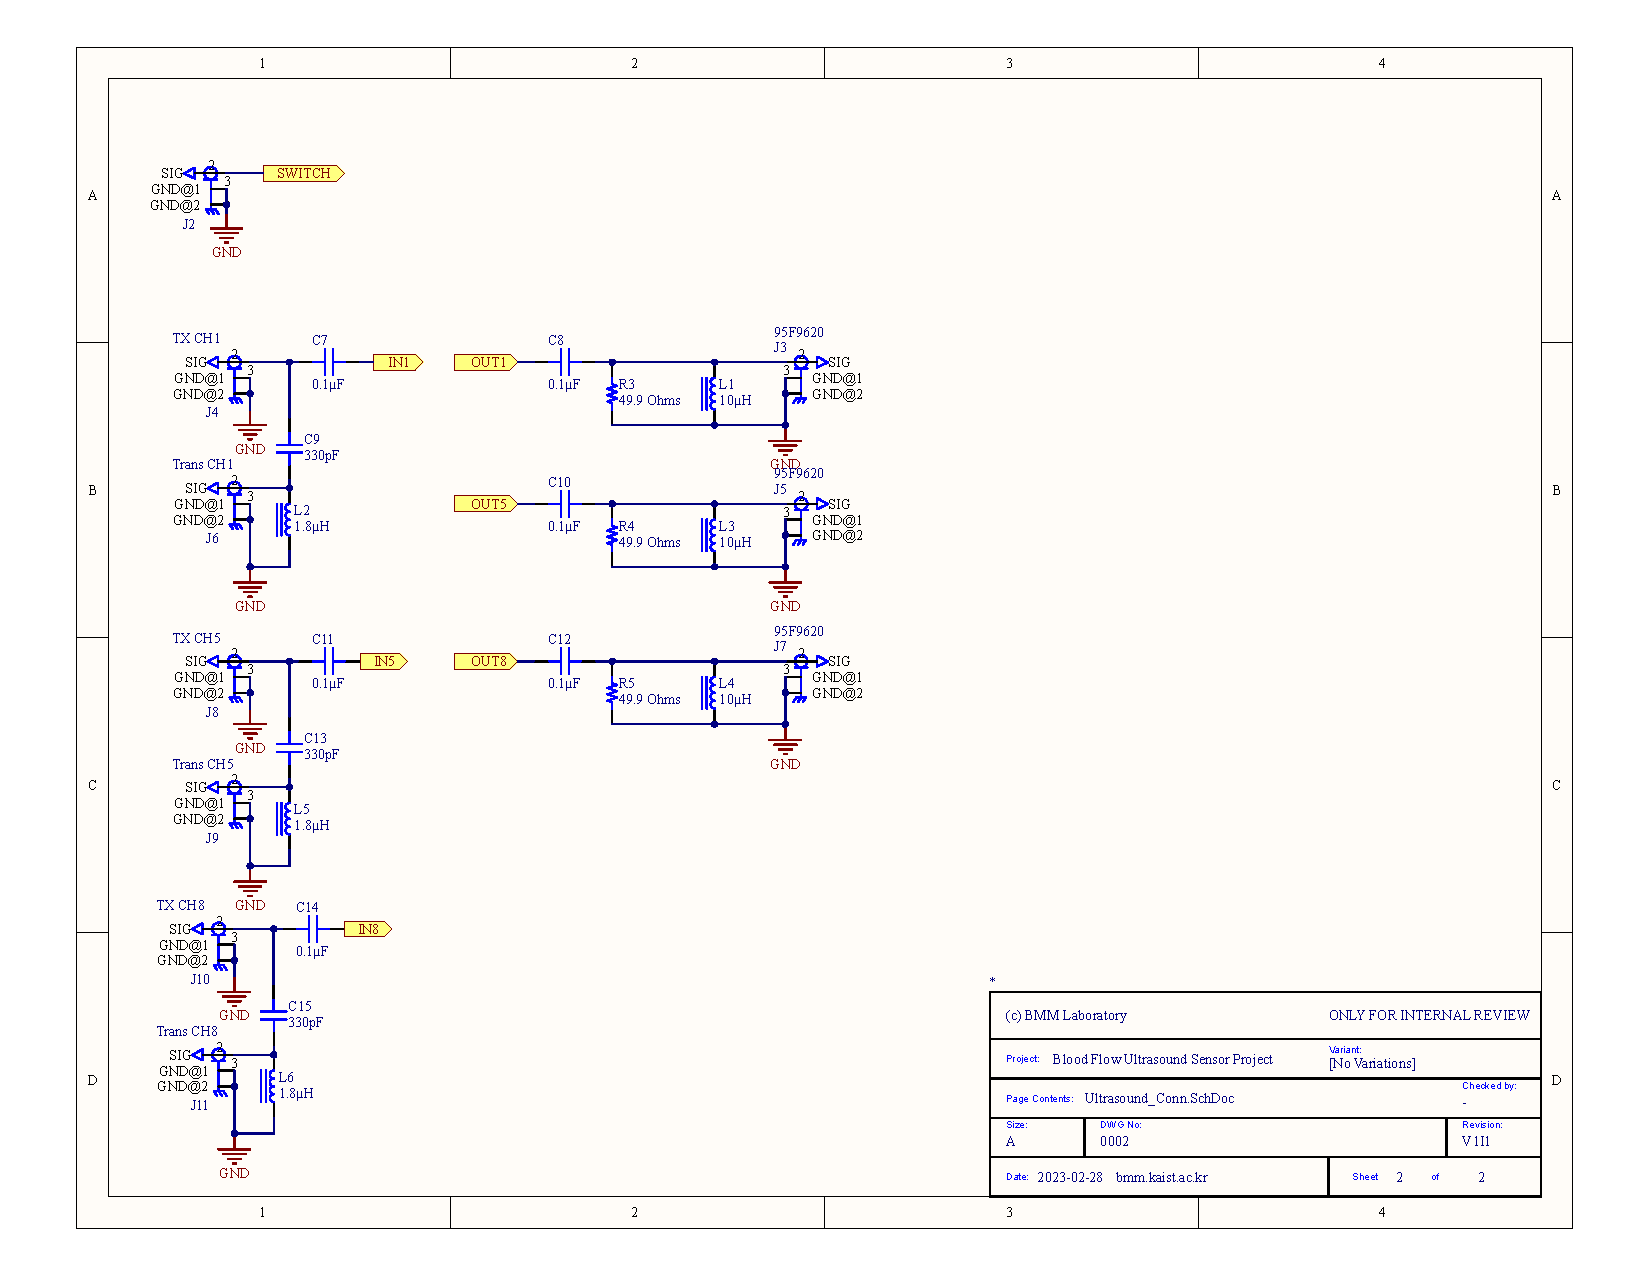
\includegraphics[width=20cm,height=28.7cm,keepaspectratio]{Figures/appendix/ultrasound_conn.pdf}
		\caption{UltrasoundSwitch Schematic B}
		\label{fig:appendix_ultrasoundswitch_b}
	\end{figure}
\end{landscape}
\begin{landscape}
	\begin{figure}[htbp]
		\centering
		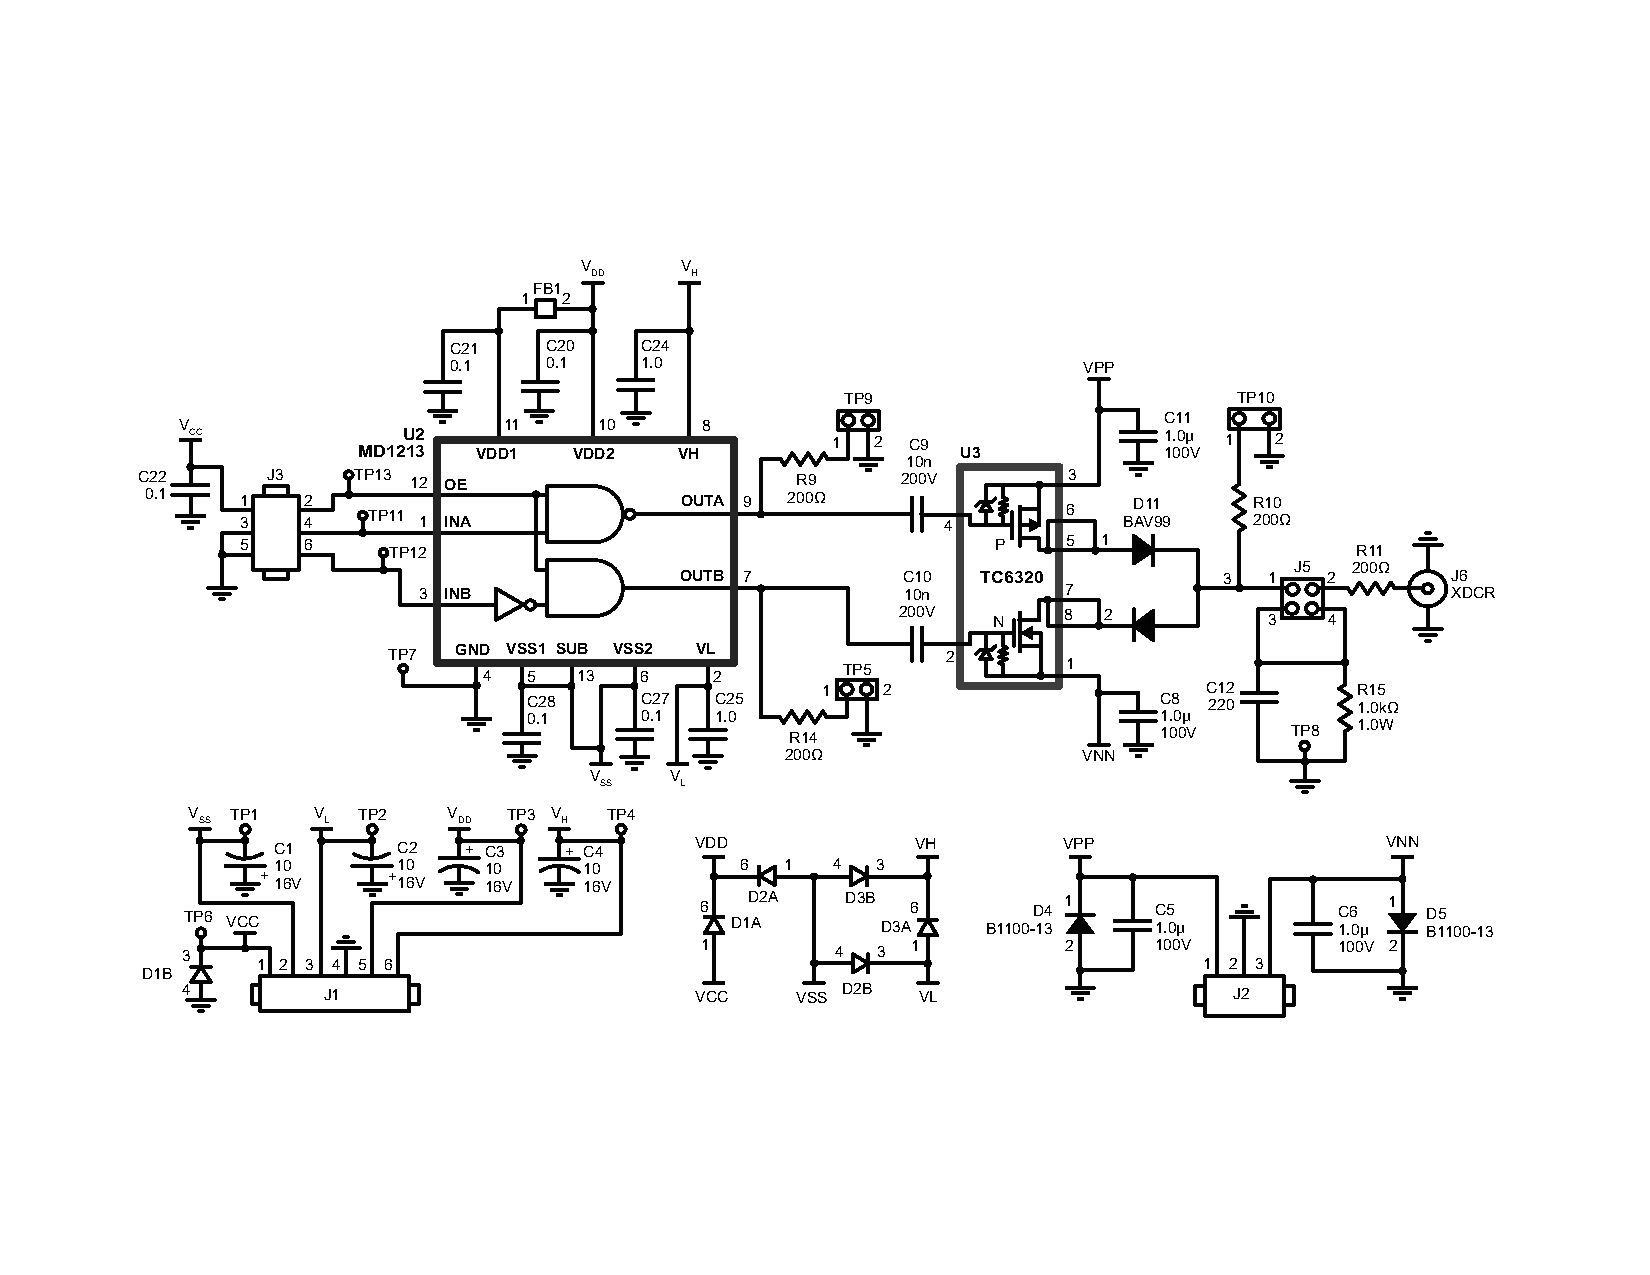
\includegraphics[width=20cm,height=28.7cm,keepaspectratio]{Figures/appendix/md1213db1_final.pdf}
		\caption{MD1213DB1 Transmitter Schematic}
		\label{fig:appendix_md1213db1}
	\end{figure}
\end{landscape}
\begin{landscape}
	\begin{figure}[htbp]
		\centering
		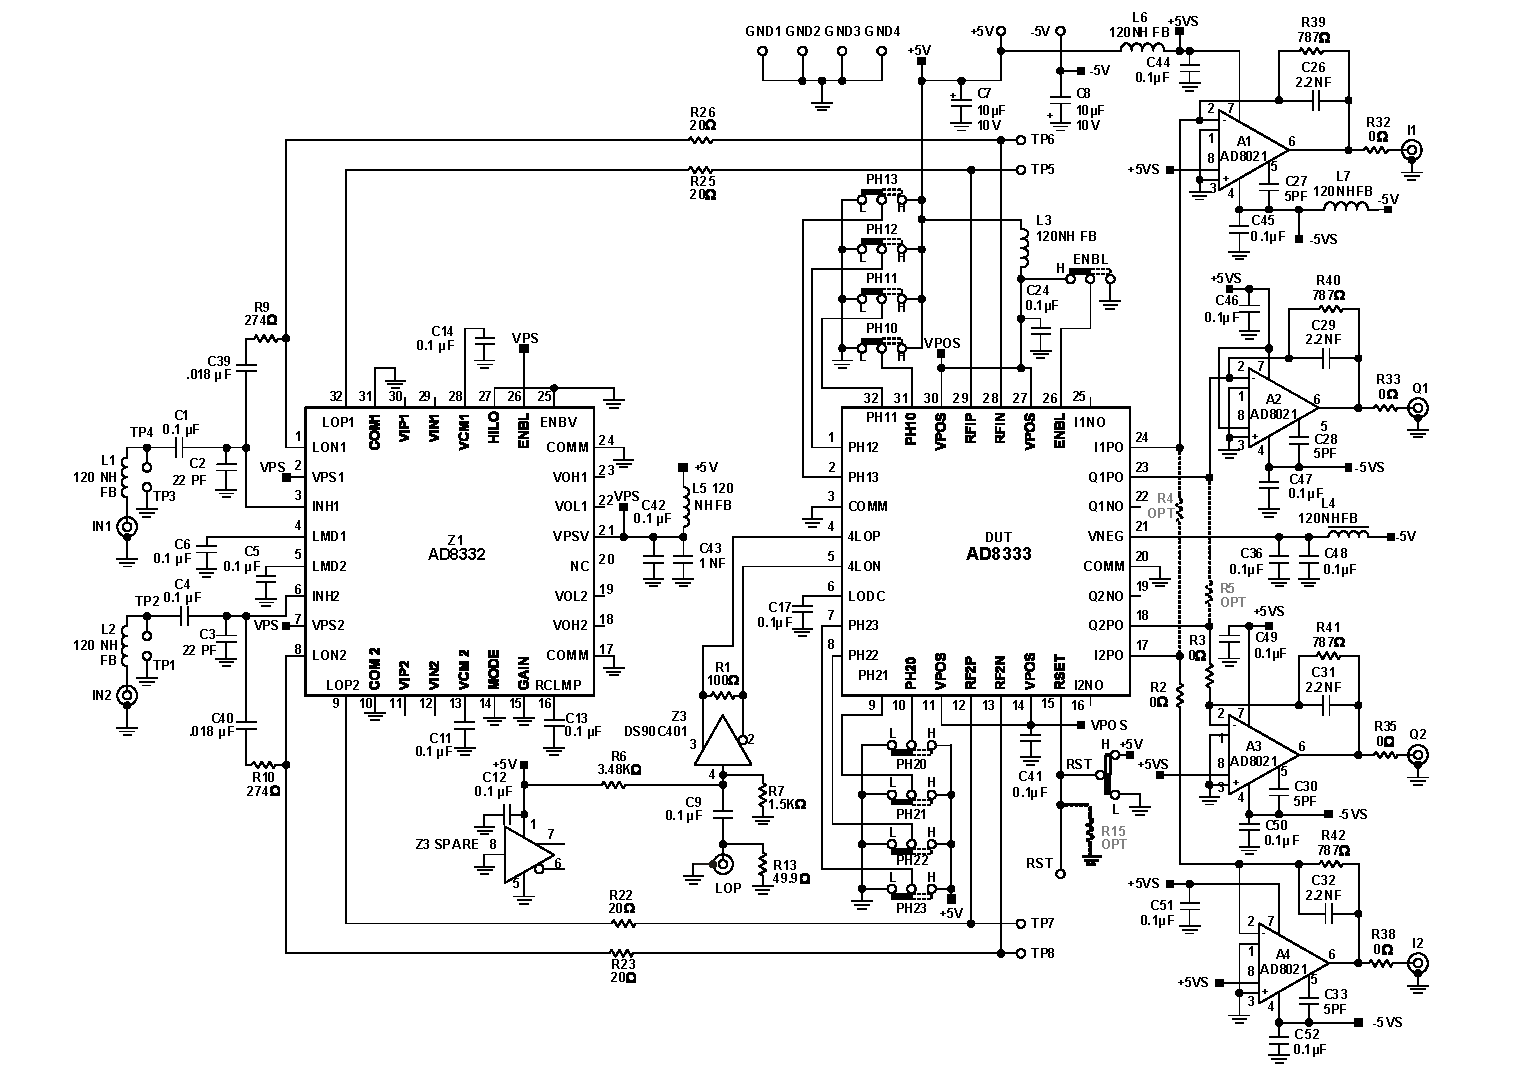
\includegraphics[width=20cm,height=28.7cm,keepaspectratio]{Figures/appendix/ad8333evalz.pdf}
		\caption{AD8332 Preamplifier, AD8333 IQ Demodulator Schematic}
		\label{fig:appendix_ad8333}
	\end{figure}
\end{landscape}
\chapter{Circuit CAD Assembly Documentation}
\begin{landscape}
	\begin{figure}[htbp]
		\centering
		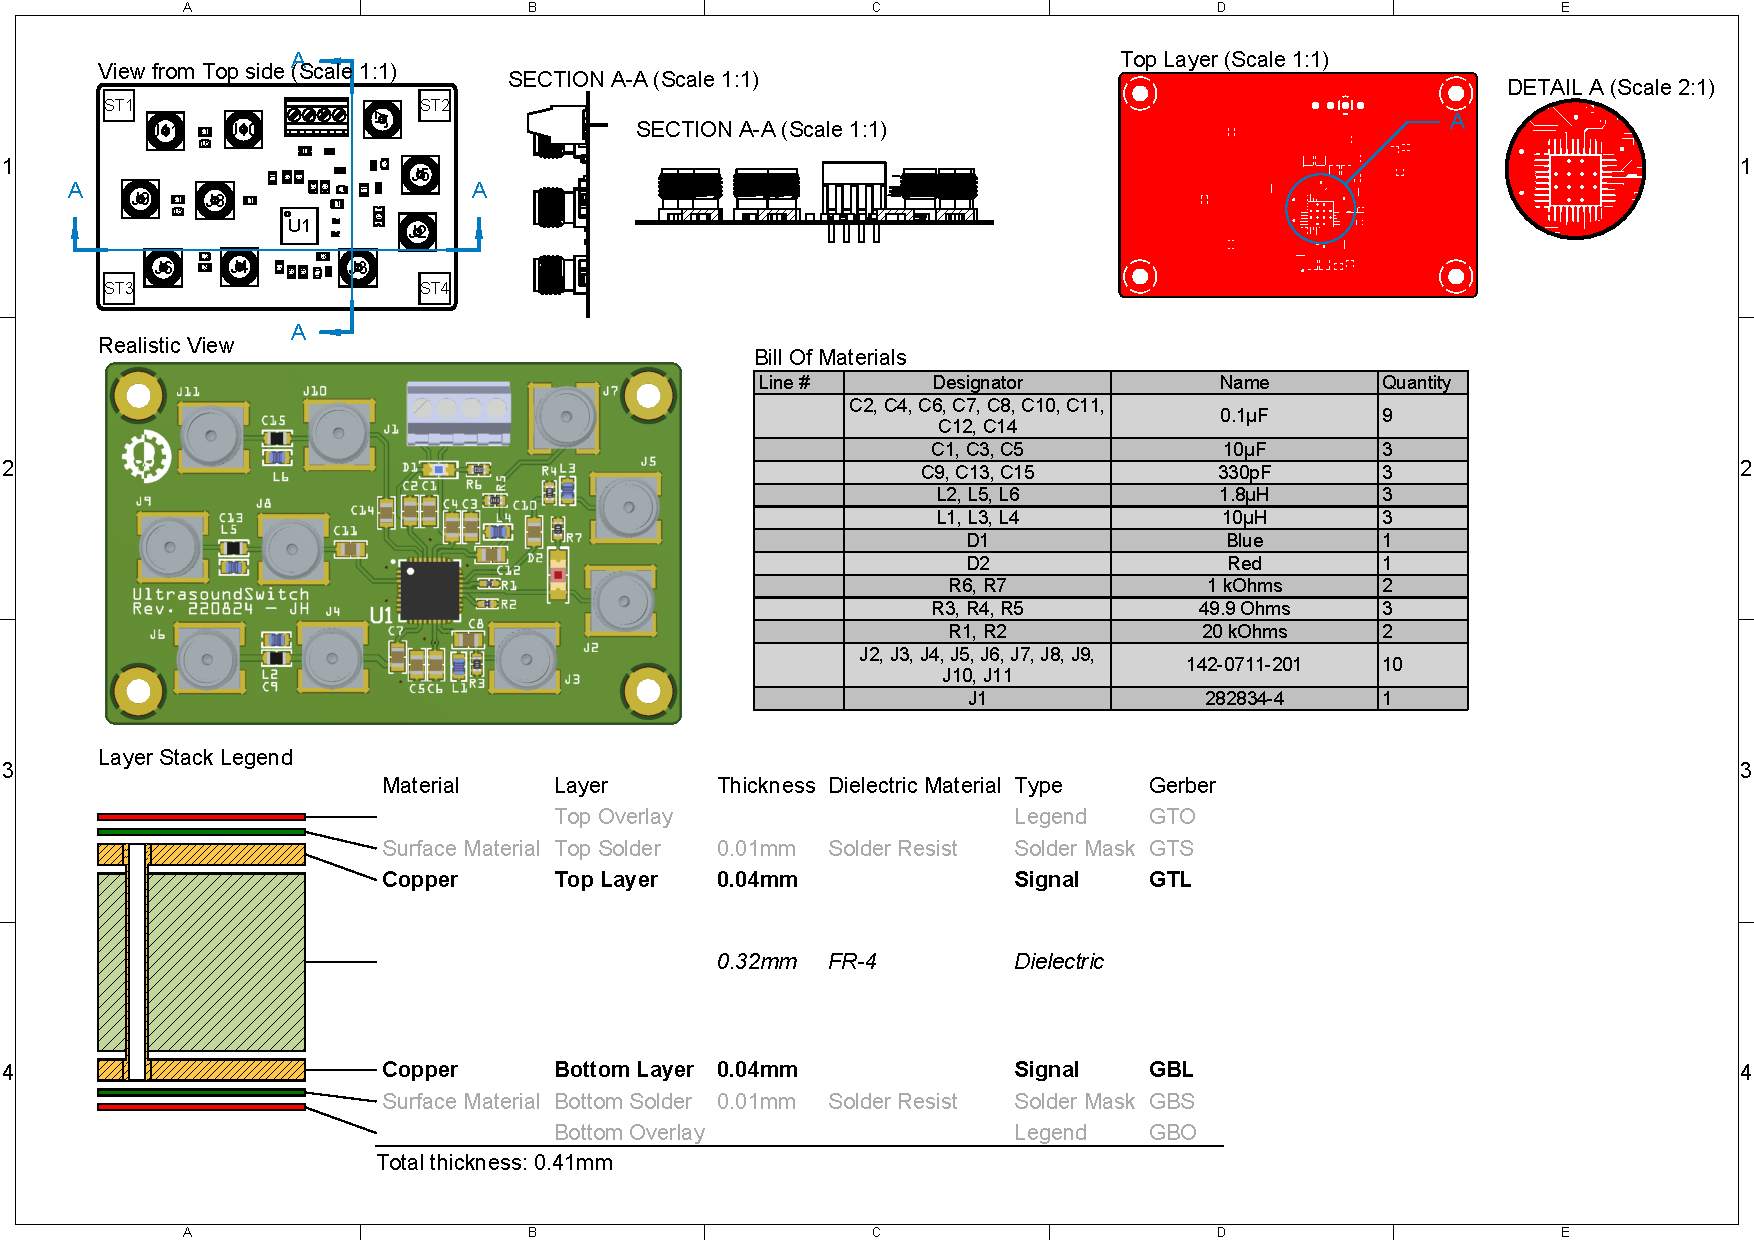
\includegraphics[width=20cm,height=28.7cm,keepaspectratio]{Figures/appendix/draftsman.pdf}
		\caption{UltrasoundSwitch Assembly Information}
		\label{fig:appendix_ultrasoundswitch_assembly}
	\end{figure}
\end{landscape}

%\chapter{Bill of Materials} \thispagestyle{main}
%
%	\begin{longtblr}[
%		%	theme=fancy,
%		caption = {Bill of Materials for the entire system},
%		entry={BOM},
%		label = {tab:bom}
%		]{
%			colspec = {lllll},
%			width = \linewidth,
%			rowhead = 1,
%%			hspan=minimal,
%			%vspan=minimal,
%		}
%		\toprule
%		{\textbf{Component}}
%		& {\textbf{Value}}
%		& {\textbf{Footprint}}
%		& {\textbf{Classification}}
%		& {\textbf{Description}}                              \\
%		\midrule
%		% table body
%		\SetCell[c=5]{c}{} Transmitter & & & & \\ \midrule
%		C1 & 1n & 0603 & X7R50V & Preamp \\
%		C13 & 1u & RAD-0.3in & Film 40V & Preamp \\
%		C14 & 1.5n & 0603 & X7R50V & PI controller \\
%		C15 & NC & 0603 & X7R50V & PI controller \\
%		C2,C3,C4 & 100n & 0603 & X7R16V & Decoupling \\
%		C5,C11 & 1u & 0603 & X5R6.3V & Decoupling \\
%		C6,C7 & 100n & 0805 & X7R50V & Decoupling \\
%		C8 & 1500u & RAD-0.3in & 63Vdc & Decoupling \\
%		P10 & 3-pin & Male & 250V & Controller bypass \\
%		P11,P12 & 10-pin & Female & 250V & InterPCB con. \\
%		P2,P3 & 1-pin header & Male & 250V & Measurements \\
%		P4,P5 & 2-way screw & NA & 300V 15A & Power,Output \\
%		P6 & 2-pin header & KK254 & 500V 4A & Audio in \\
%		P7 & 4-pin header & Female & 250V & 5V Power \\
%		P8,P9 & BNC & PCB & 500V & Audio in, Output \\
%		R2 & 16.2k & 0603 & 1\% & Preamp \\
%		R1,R3 & 2k & 0603 & 1\% & Preamp \\
%		R4,R7 & 4.75k & 0603 & 1\% & Voltage ref \\
%		R5 & 33.2k & 0603 & NA & PI controller \\
%		R6 & 0 (short) & 0603 & NA & PI controller \\
%		R9 & 0 (short) & 0603 & NA & PI controller \\
%		R10 & NC & 0603 & NA & PI controller \\
%		R8 & 2.49k & 0603 & 1\% & Voltage ref \\
%		U1 & OPA2365 & SOIC-8 & NA & Preamp, PI \\
%		U2 & TLV431A & SOT-23 & 1\% & Voltage ref \\ %\pagebreak
%		\SetCell[c=5]{c}{} Receiver & & & & \\ \midrule
%		C1,C11,C15 & 100n & 0603 & X7R16V & Gate driver \\
%		P1,P2 & 10-pin header & Male & 250V & InterPCB con. \\
%		C2,C16 & 150n & 0603 & X5R10V & Gate driver \\
%		C3,C10 & 100p & 0603 & NPO50V & Decoupling \\
%		L1,L2 & 1.768u & Radial & NA & Output filter \\
%		U1,U3 & LM5113 & WSON-10 & NA & Gate driver \\
%		R20 & 15m sense & 1210 & 1\% 1W & Output filter \\
%		R1,R6 & 500 & 3213 & NA & Gate driver \\
%		Q1,Q2,Q3,Q4 & BSZ097-N10NS5 & TSDSON-8 & NA & Power stage \\
%		R2,R5,R8,R10 & 5 & 0603 & 1\% & Gate driver \\
%		R4,R9 & 0 & 0603 & 1\% & Gate driver \\
%		D1,D2 & Diode & NA & 85V 0.25A & Gate driver \\
%		C5,C6,C9,C17 & 10u & 1210 & X7R50V & Decoupling \\
%		C12,C13,C14 & 680n & 1210 & X7R100V & Output filter \\
%		\SetCell[c=5]{c}{} Microcontroller & & & & \\ \midrule
%		C18,C20,C27 & 100n & 0603 & X7R16V & Decoupling \\
%		C28,C29 & 100n & 0603 & X7R16V & Decoupling \\
%		U6 & LT1999 & MSOP-8 & NA & Current acq. \\
%		U4 & AD8274 & MSOP-8 & NA & Volt acq. \\
%		U2 & LT1711 & MSOP-8 & NA & AIM \\
%		C4 & NC & 0603 & X7R16V & AIM \\
%		C7 & NC & 0603 & X7R16V & AIM \\
%		C8 & NC & 0603 & X7R16V & Cur. acq. \\
%		CA1 & 1.5n & 0603 & X7R50V & AIM \\
%		R14 & 8.66k & 0603 & 1\% & AIM \\
%		R18 & 16.2k & 0603 & 1\% & AIM \\
%		R23 & 1.5k & 0603 & 1\% & AIM \\
%		R3,R11 & 120k & 0603 & 1\% & Voltage acq. \\
%		RA1 & 2.2k & 0603 & 1\% & AIM \\
%		RA2 & 20k & 0603 & 1\% & AIM \\
%		RA3 & 2.74k & 0603 & 1\% & AIM \\
%		RA4 & 0 & 0603 & NA & AIM \\
%		\bottomrule
%	\end{longtblr}

\chapter{Instruments} \thispagestyle{main}
\begin{table}[ht]
	\centering
	\caption{List of instruments used for solder work}
	\label{tab:instruments_solder_work}
	\begin{tblr}[]{%
			colspec = {lll},
			row{1} = {guard, m, font=\small\bfseries},
		}
		\toprule
		Function & Manufacturer & Model \\ \midrule
		Visual inspection microscope & Leica & A60 \\
		Manual soldering & Weller & WX2 \\
		Heat gun & Thermaltronics & TMT-HA600-2 \\
		Solder paste & Chip Quik & SMD291AX250T3 \\
		Solder flux & Chip Quik & SMD291NL \\
		Reflow oven & Puhui & T-962A \\
		DMM & Fluke & 175 \\ \bottomrule
	\end{tblr}
\end{table}

\begin{table}[ht]
	\centering
	\caption{List of instruments used in experiments}
	\label{tab:instruments_hardware}
	\begin{tblr}[]{%
			colspec = {lll},
			row{1} = {guard, m, font=\small\bfseries},
		}
		\toprule
		Function & Manufacturer & Model \\
		\midrule
		DCPS 1 & RIGOL & DP832A 200W \\
		DCPS 2 & Keysight & E3631A 80W \\
		Function generator 1 & Keysight & 33500B \\
		Function generator 2 & Tektronix & AFG3102 \\
        DMM & Fluke & 175 \\
		Transducer (PZT) & HAGISONIC & M715-SB-S 204 \qty{5}{\mega\hertz} \\
		Transducer (CMUT) & BMM Creation & 6ch \qty{3.3}{\mega\hertz} C.F. \\
		RF Amplifier & Tomco & BT00100-AlphaS-CW \\
		Oscilloscope 1 & Keysight & DSO-X 2024A \\
		Oscilloscope 2 & Tektronix & MSO4054 \\
		Physiological simulator & CIRS & Doppler String Phantom 043A \\
		Vector Network Analyzer & Agilent & E5071B ENA Series Network Analyzer \\
		\bottomrule
	\end{tblr}
\end{table}

%\chapter{Embedded}
%\subsection{Zephyr}
%Zephyr is an \gls{open-source} \gls{rtos} designed to be lightweight and run on a wide range of devices, from \gls{mcu}s with as little as \qty{20}{\kilo\byte} of \gls{ram} to more powerful systems with multiple processors. Zephyr is designed to be modular and scalable, with a focus on security and low power consumption. It includes support for a wide range of hardware architectures, including ARM Cortex-M, x86, and RISC-V, and it can be used with a variety of development boards and microcontrollers. One of the key features of Zephyr is its ability to run on very small devices with limited resources. It includes support for various networking protocols, such as \gls{ble}, IPv4, and IPv6, which makes it well-suited for use in \gls{iot} applications. Zephyr is developed as part of the Linux Foundation's Zephyr Project, and it is widely used in the development of IoT and embedded systems.
%
%\subsubsection{Build System}
%To build an application with the Zephyr kernel, you use CMake which has two phases - configuration and build. During configuration phase, CMake executes the \texttt{CMakeLists.txt} build scripts to generate an internal model of the Zephyr build. Starting with \gls{dts} and \gls{dtsi} and then using the device-tree nodes and Kconfig to configure the set of build files for ninja.
%\begin{figure}[htbp]
%	\centering
%	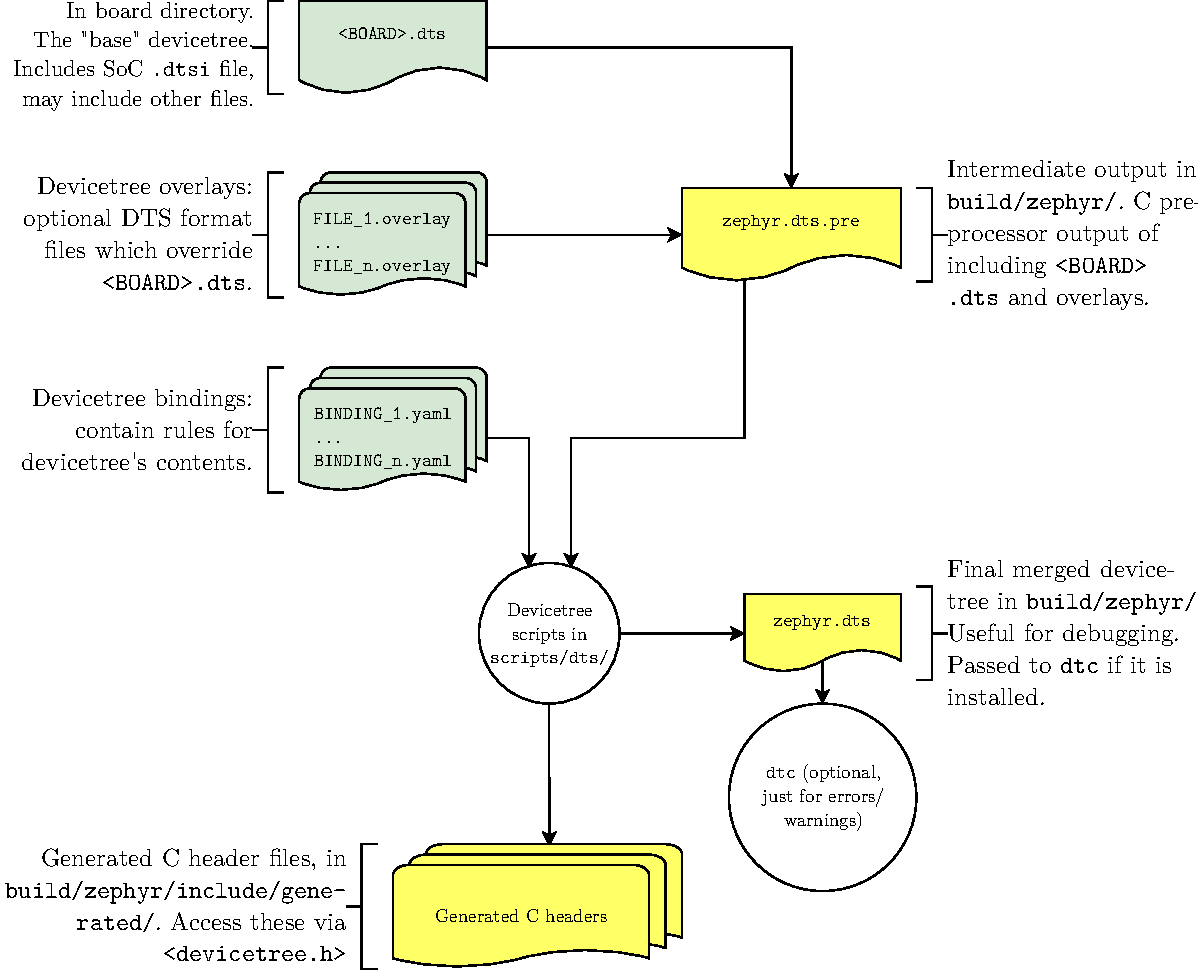
\includegraphics[width=.8\textwidth]{Figures/3_devicetree.pdf}
%	\caption[Devicetree input files and output files]{Devicetree input files (green) and output files (yellow) \cite{zephyrprojectdocumentation}}
%	\label{fig:3_devicetree}
%\end{figure}
%Seen in \cref{fig:3_devicetree} is the process in which the build system searches out device-trees in certain locations and merges them into the \texttt{zephyr.dts} that will be used for configuring and mapping every peripheral. Typically, each supported board has a file called \texttt{BOARD.dts} that defines the hardware of the board. The \texttt{BOARD.dts} file includes one or more \texttt{.dtsi} files that describe the CPU or system-on-chip that Zephyr runs on, and other common hardware features shared by multiple boards. These \texttt{.dtsi} files may also include other \texttt{.dtsi} files. Additionally, the \texttt{BOARD.dts} file provides a description of the specific hardware of the board. After parsing the \texttt{BOARD.dts} file, the main point being the merge with the \texttt{.overlay} file specific to both the project and the board. This overlay enables the portability feature of Zephyr. A significant degree of the workload when implementing Zephyr projects are thus in writing hardware devicetrees and then writing as generic firmware implementations as possible. Next, the configuration phase can be seen in \cref{fig:3_cmake_configuration}. Once configuration phase is done, CMake generates build scripts that are native to the host platform and initiate the build sequence with the build system Ninja \cite{ninja}. Afterwards, the generated build scripts are executed to begin the second phase, build. The build scripts can recompile the application without involving CMake after most code changes. Zephyr uses the \enquote{target} concept of CMake to organize the build, where a target can be an executable, a library, or a generated file. The final output of Ninja is a binary file ready for \gls{flashing} using a microcontroller programmer.
%
%\begin{figure}[htbp!]
%	\centering
%	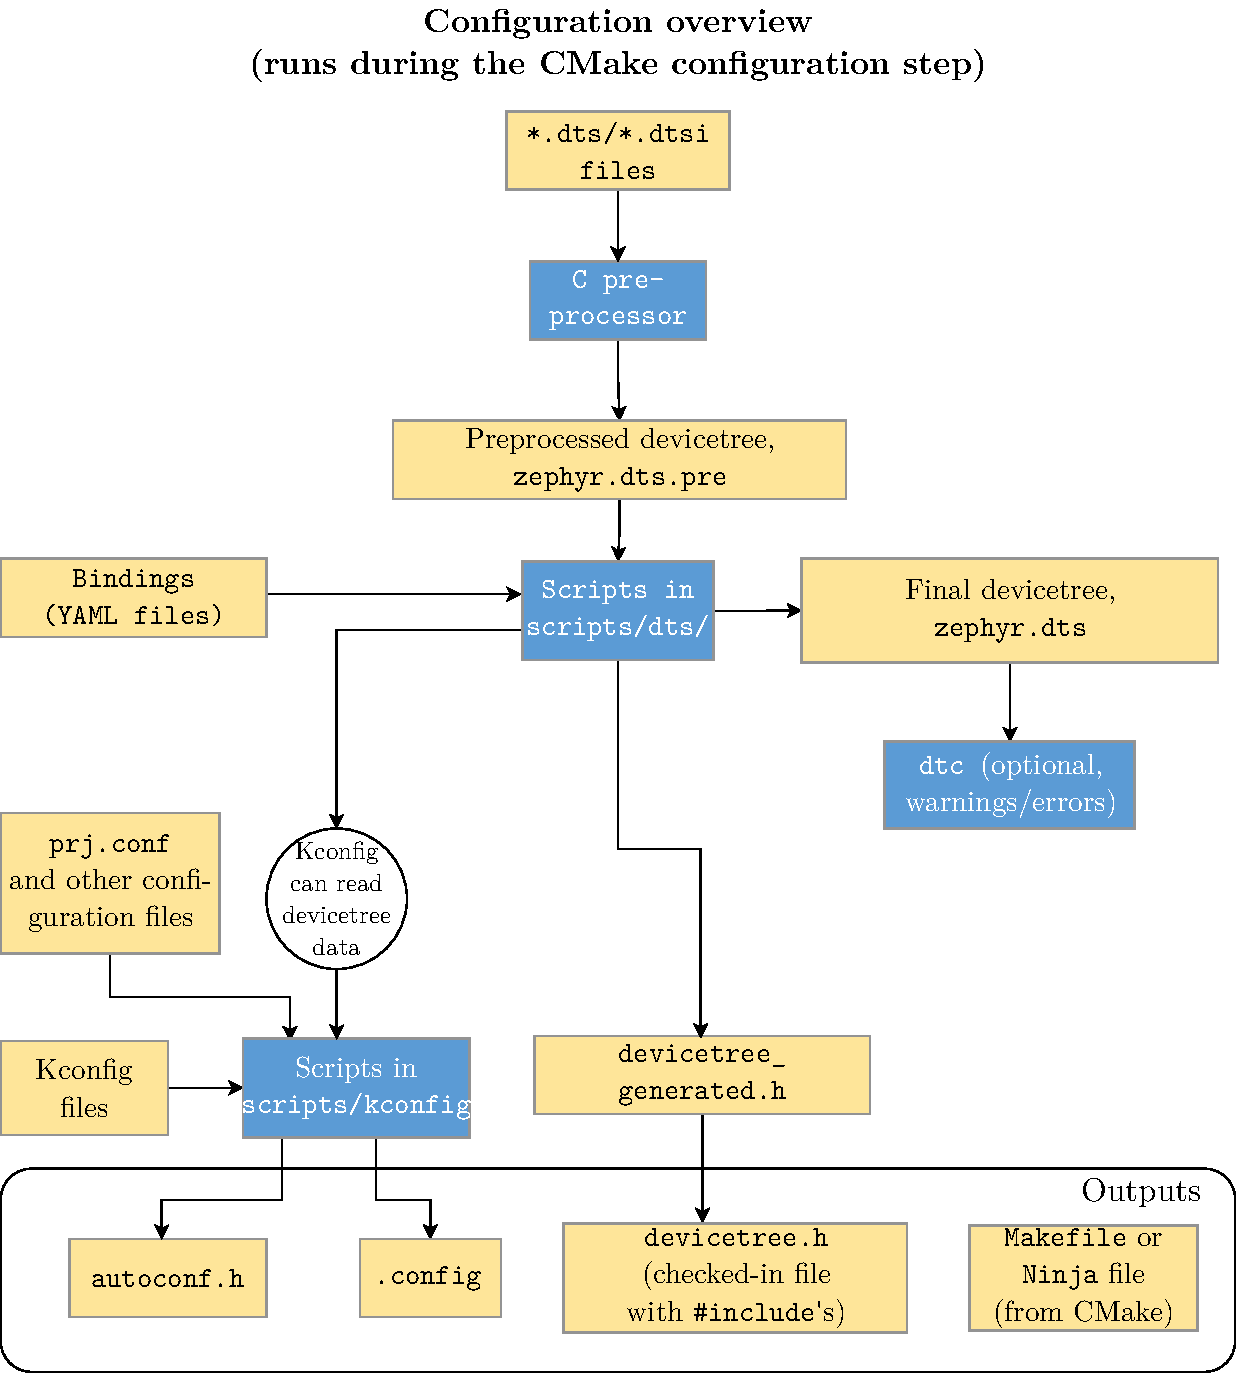
\includegraphics[width=.8\textwidth]{Figures/3_cmake_configuration.pdf}
%	\caption[Configuration phase of a Zephyr application]{Configuration phase of a Zephyr application \cite{zephyrprojectdocumentation}}
%	\label{fig:3_cmake_configuration}
%\end{figure}
%After cmake configuration phase has completed, the build phase begins. CMake invokes the build system, which (conceptually) has five (six, one is repeated) stages: (I) pre-build, (II) generation and compilation, (III) first-pass binary (and (IV) second-pass binary), (V) final binary and (VI) post-processing.
%\begin{figure}[htbp]
%	\centering
%	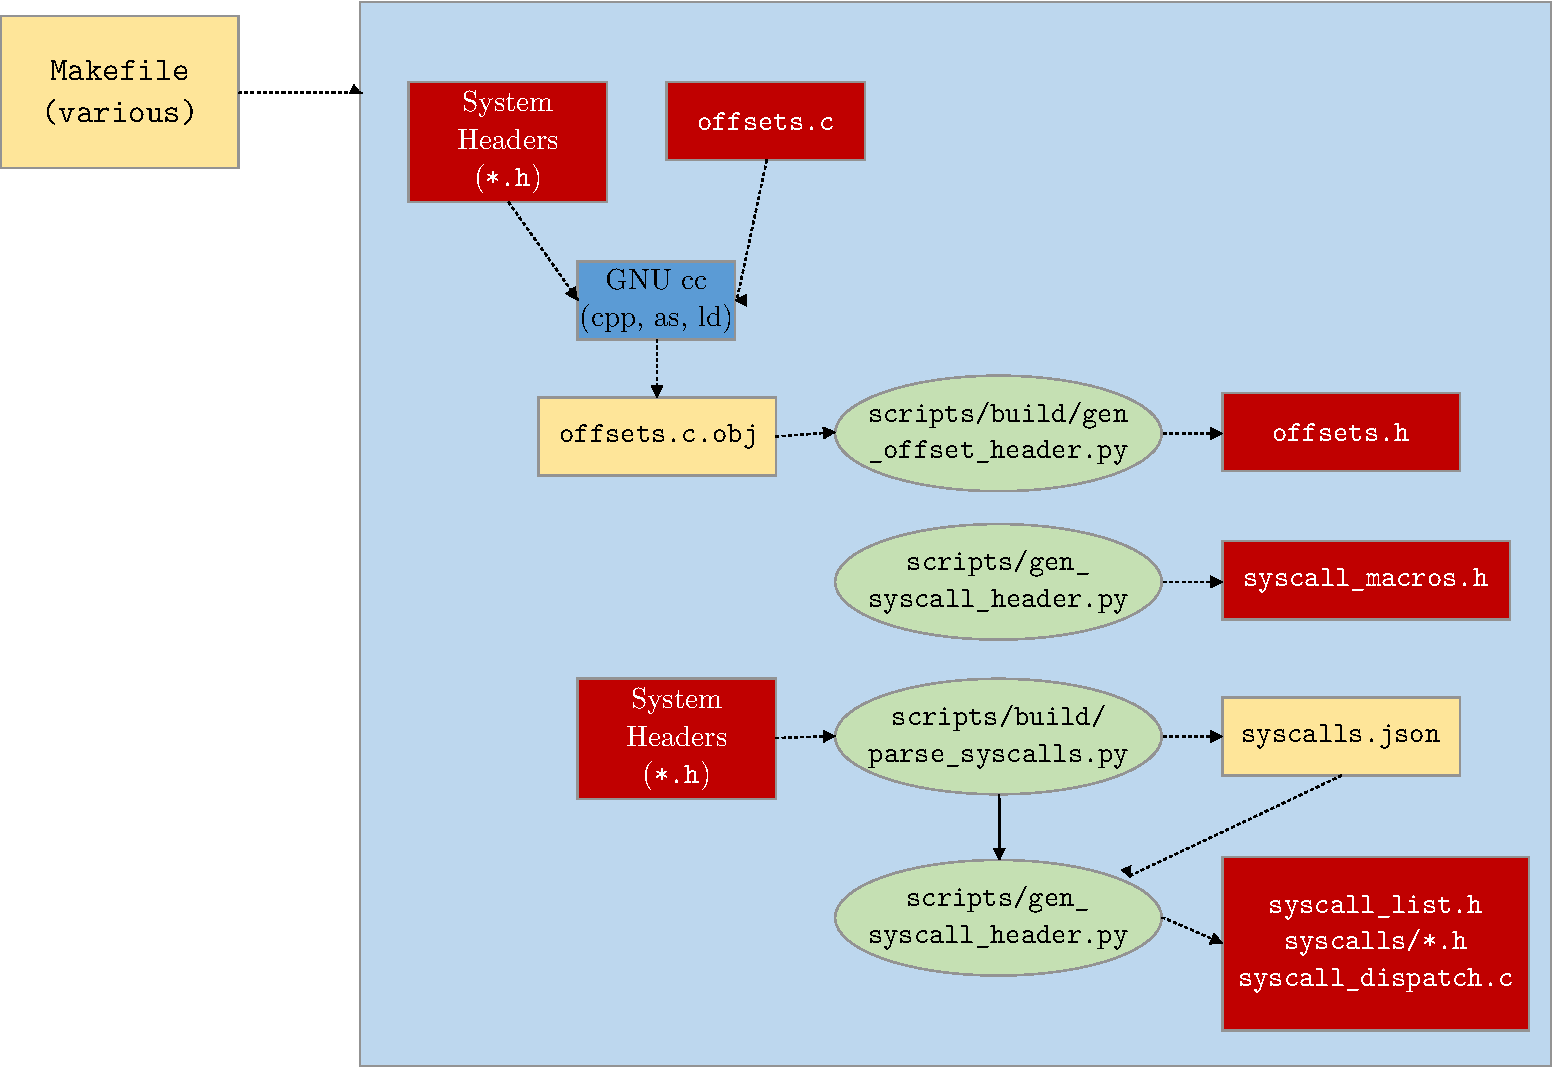
\includegraphics[width=.8\textwidth]{Figures/3_cmake_build1.pdf}
%	\caption[Flowchart of build stage I, pre-build]{Flowchart of build stage I, pre-build}
%	\label{fig:3_build1}
%\end{figure}
%In \cref{fig:3_build1} the build system binds system call functions to implementations.
%\begin{figure}[htbp]
%	\centering
%	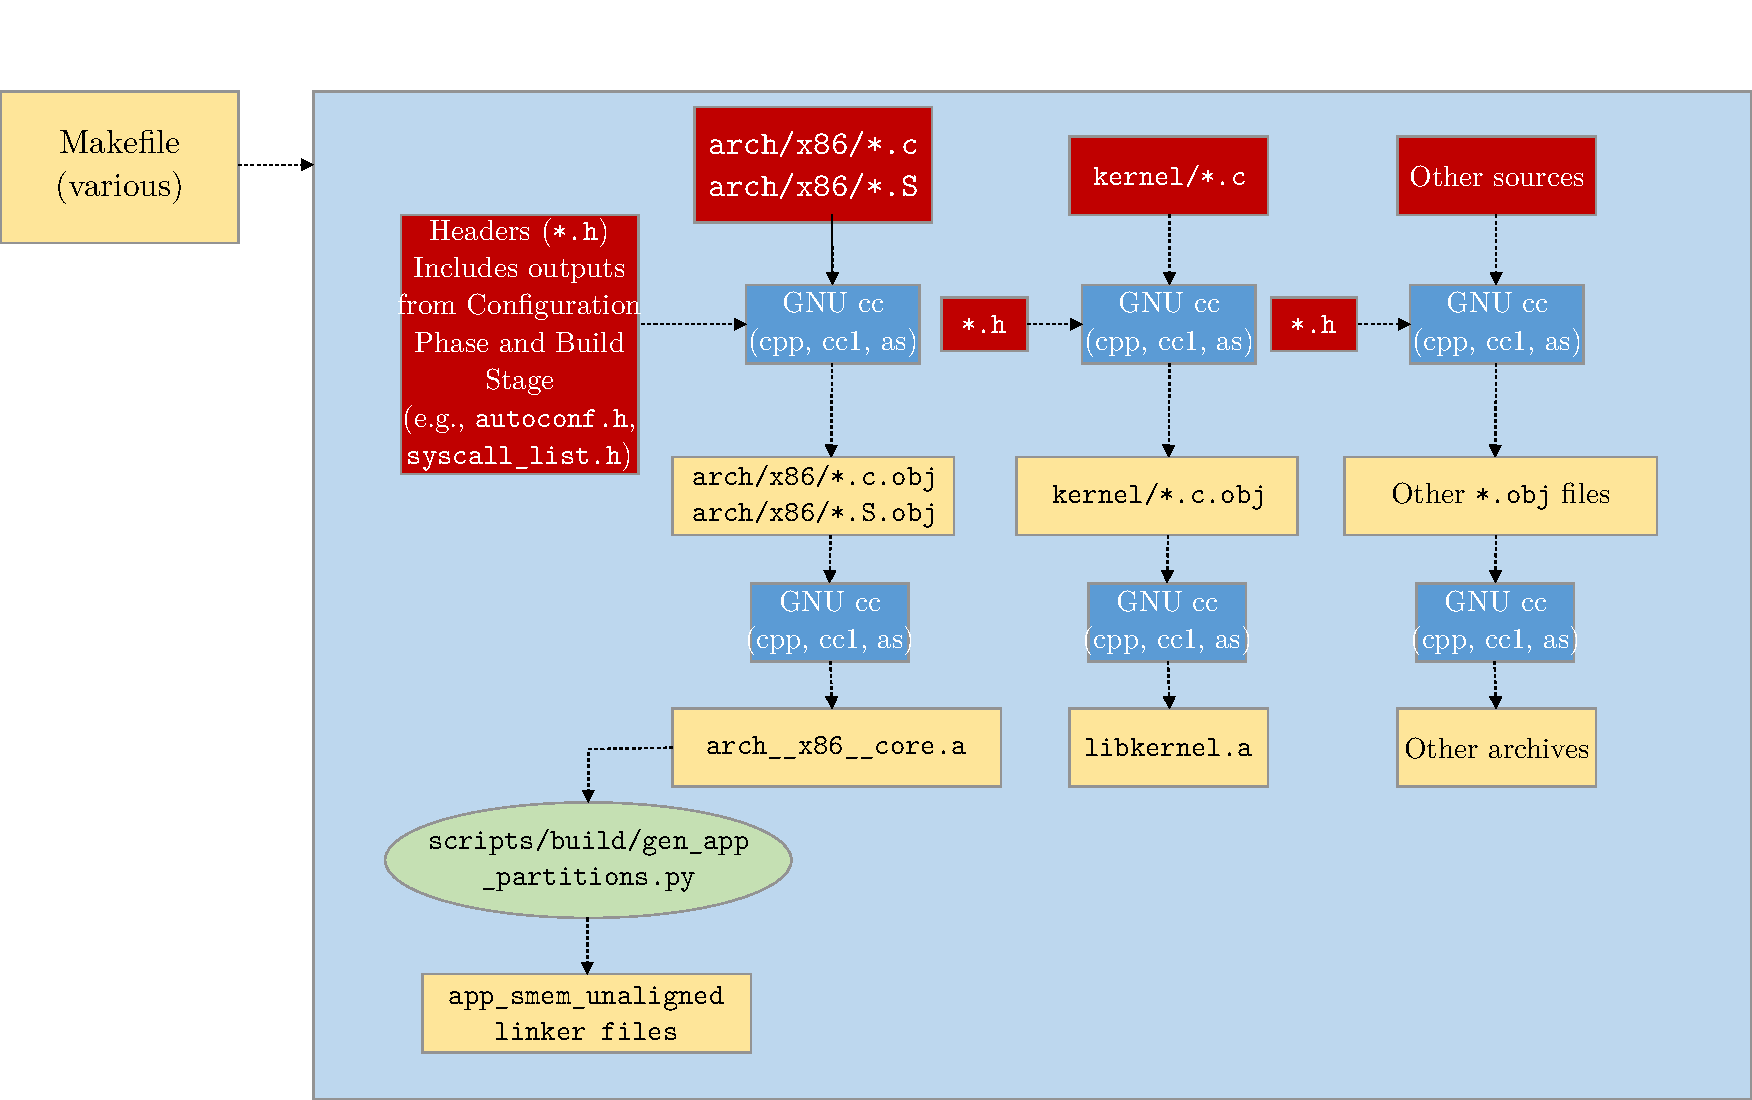
\includegraphics[width=.8\textwidth]{Figures/3_cmake_build2.pdf}
%	\caption[Flowchart of build stage II, generation and compilation]{Flowchart of build stage II, generation and compilation}
%	\label{fig:3_build2}
%\end{figure}
%Next, in \cref{fig:3_build2} the build system collects source files for various subsystems (decided by the configuration phase) and compiles into archives. The \texttt{gen\_app\_partitions.py} script examines all the archives that are produced and creates linker scripts that organize and align application partitions correctly, based on the memory protection hardware of the target. Then \texttt{cpp} process involves merging linker script fragments from various sources, including the target's architecture/\gls{soc}, the kernel tree, partition output (if memory protection is enabled), and any other selected fragments from the configuration process. These are combined into a \texttt{linker.cmd} file. The compiled archives are then linked with \texttt{ld}, following the specifications in the \texttt{linker.cmd} file.
%\begin{figure}[htbp]
%	\centering
%	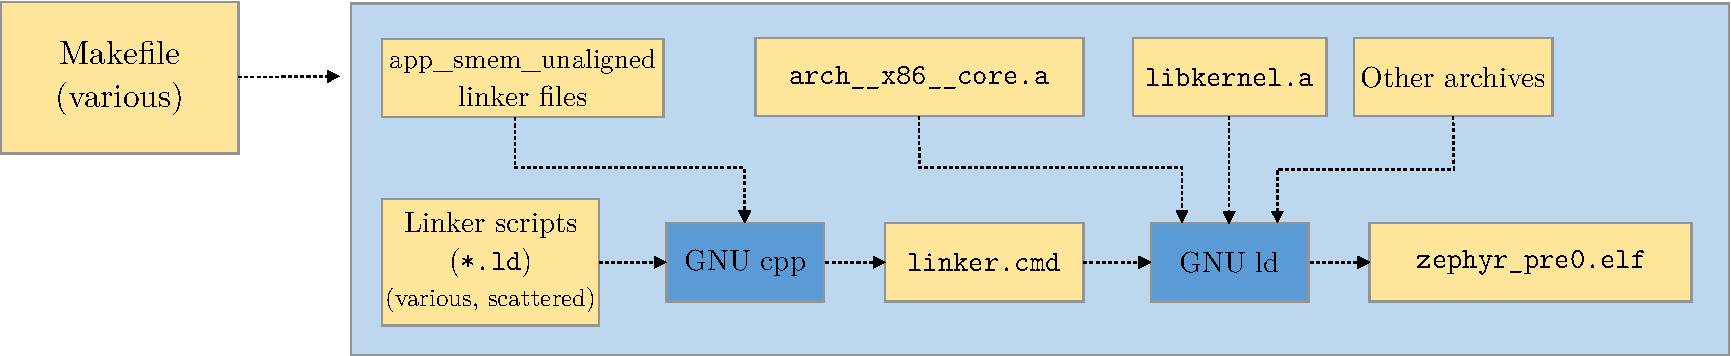
\includegraphics[width=.8\textwidth]{Figures/3_cmake_build3.pdf}
%	\caption[Flowchart of build stage III, intermediate binary]{Flowchart of build stage III, intermediate binary}
%	\label{fig:3_build3}
%\end{figure}
%Shown in \cref{fig:3_build3} is the process, in which an unfixed size intermediate binary is produced. If a devicetree is being used, an intermediate binary is generated that has a variable size. The binary is not fixed in size, which means that it can be modified by post-processing steps that affect the size of the final binary.
%\begin{figure}[htbp]
%	\centering
%	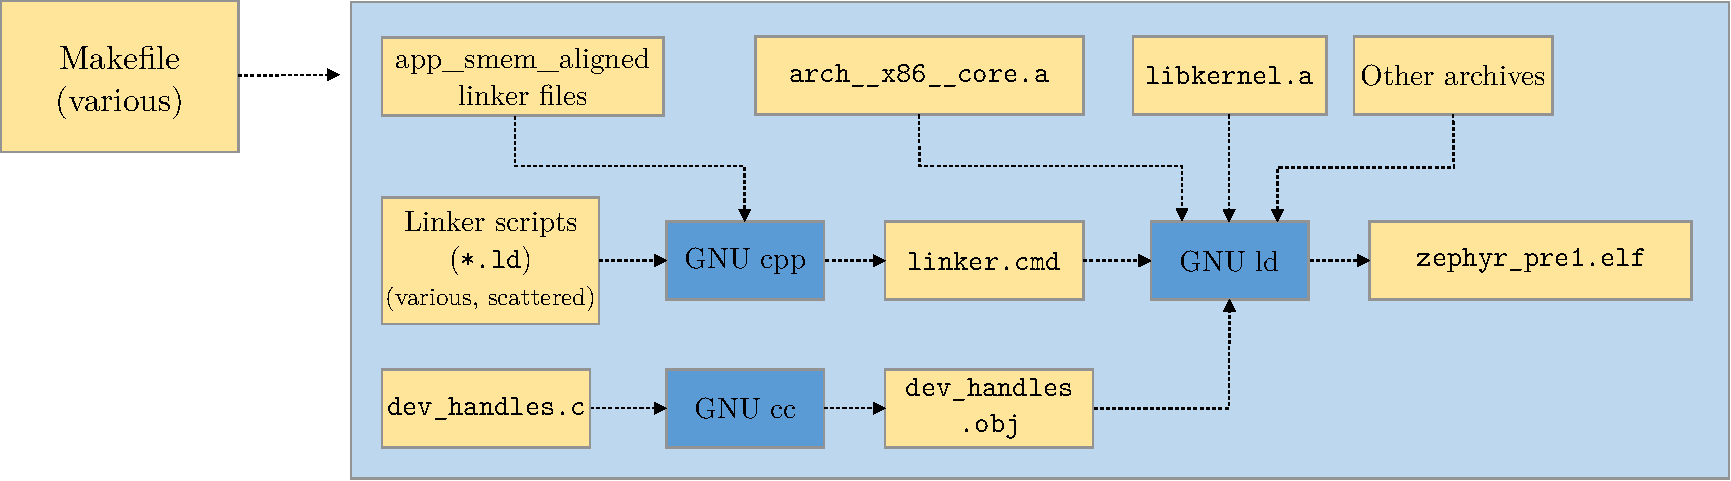
\includegraphics[width=.8\textwidth]{Figures/3_cmake_build4.pdf}
%	\caption[Flowchart of build stage IV, second intermediate binary]{Flowchart of build stage IV, second intermediate binary}
%	\label{fig:3_build4}
%\end{figure}
%In \Cref{fig:3_build4} the fixed size intermediate binary is generated. The previous stage's binaries are not fully formed and contain sections that are empty or marked as placeholders. These sections must be filled in by a process similar to reflection. To finish building, certain scripts are run on the intermediate binaries. These scripts generate the necessary components that are missing from the final binary.
%\begin{figure}[htbp]
%	\centering
%	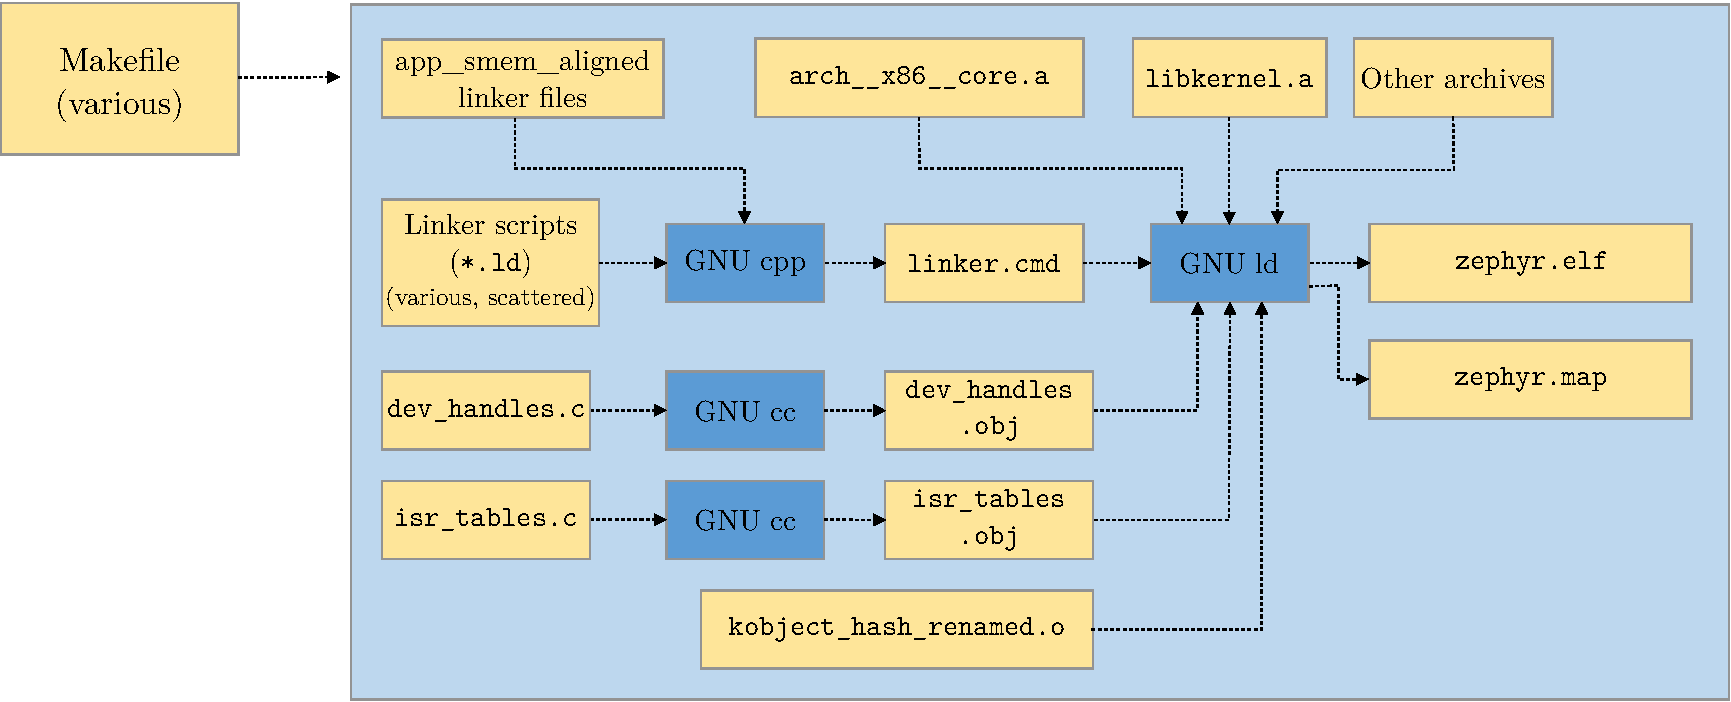
\includegraphics[width=.8\textwidth]{Figures/3_cmake_build5.pdf}
%	\caption[Flowchart of build stage V, final binary]{Flowchart of build stage V, final binary}
%	\label{fig:3_build5}
%\end{figure}
%Next, in \cref{fig:3_build5}, the final binary is produced by repeating the link from the previous stage, but this time with all the missing pieces populated.
%\begin{figure}[htbp]
%	\centering
%	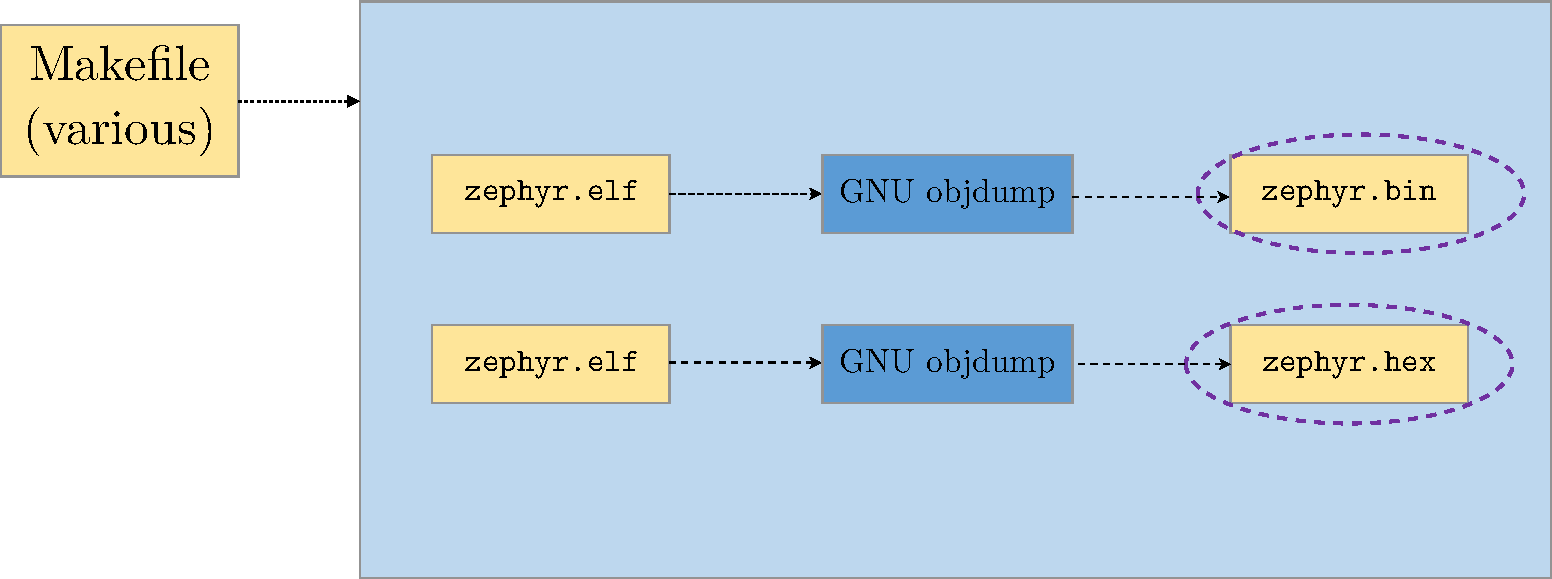
\includegraphics[width=.6\textwidth]{Figures/3_cmake_build6.pdf}
%	\caption[Flowchart of build stage VI, post-processing]{Flowchart of build stage VI, post-processing}
%	\label{fig:3_build6}
%\end{figure}
%Finally, in \cref{fig:3_build6}, using \texttt{GNU objdump}, the completed kernel is converted from a \gls{elf} file to the hex file that is expected by the flash tool compatible with the target device.

%\subsection{Firmware}
%A full repository of the revision controlled codebase is available on GitHub at \cite{github_firmware}.